\documentclass[11pt, a4paper]{article}
\usepackage[T1]{fontenc}
\usepackage{mwe}
\usepackage[margin=3.5cm]{geometry}
\usepackage{amsmath}
\usepackage{amssymb}
\usepackage{bm} % for bold vectors in math mode
\usepackage{physics} % many useful physics commands
\usepackage[separate-uncertainty=true]{siunitx} % for scientific notation and units

\usepackage{graphicx}
\graphicspath{{"../figures/"}}
\usepackage[section]{placeins} % to keep figures in their sections
\usepackage[export]{adjustbox} % for subcaptionbox figures

\usepackage[most, minted]{tcolorbox} % for displaying code

\usepackage{xcolor}  % to color hyperref links
\usepackage[colorlinks = true, allcolors=blue]{hyperref}


\setlength{\parindent}{0pt} % to stop indenting new paragraphs
\newcommand{\diff}{\mathop{}\!\mathrm{d}} % differential
\newcommand{\F}{\mathcal{F}} % Fourier transform

\newcommand{\acov}{\operatorname{autocov}}
\newcommand{\avar}{\operatorname{autovar}}

\newcommand{\eqtext}[1]{\qquad \text{#1} \qquad}



\newtcblisting{python}{%
	listing engine=minted,
	minted language=python,
	listing only,
	breakable,
	enhanced,
	minted options = {
		linenos, 
		breaklines=true, 
		tabsize=2,
		fontsize=\footnotesize, 
		numbersep=2mm
	},
	overlay={%
		\begin{tcbclipinterior}
			\fill[gray!25] (frame.south west) rectangle ([xshift=4mm]frame.north west);
		\end{tcbclipinterior}
	}   
}



\begin{document}
\title{Cross-Correlation and the Fast Fourier Transform}
\author{Elijan Jakob Mastnak\\[1mm]\small{Student ID: 28181157}}
\date{November 2020}
\maketitle

%\textit{Please forgive the perhaps excessive report length---the large number of pages is largely due to figures and code, which should read quickly.}

\tableofcontents

\vspace{5mm}
\textit{Note}: All text in \textcolor{blue}{blue} is a clickable hyperlink for easier document navigation.

\newpage
\begin{center}
\textbf{Assignment}
\begin{enumerate}
	\item Analyze the various recordings of two great horned owls' calls found on the course website.  Using autocorrelation and cross-correlation, compare the signals among each other, and identify which owl is heard in each recording. 
	
	\item \textit{Optional:} Use cross-correlation and autocorrelation to analyze some other signal(s), either ones you record on your own or some other periodic signals from an existing database.
\end{enumerate}
\end{center}

\vspace{2mm}

\rule{\textwidth}{0.2pt}

\section{Theory} \label{fft:s:theory}
\vspace{-2mm}
\textit{To jump right to the solution, see \hyperref[fft:s:solution]{Section \ref{fft:s:solution}}}.

\subsection{Cross-Correlation}
The cross-correlation of two periodic signals $ f(t) $ and $ g(t) $, both with period $ T $, is defined as
\begin{equation*}
	\phi_{fg}(\tau) = \frac{1}{T}\int_{0}^{T}f(t + \tau)g(t) \diff t
\end{equation*}
The analogous discrete version, for two discrete signals $ \{f_{k}\} $ and $ \{g_{k}\} $ where $ k = 0, 1, \ldots, N -1 $ is
\begin{equation*}
	\phi_{fg}(n) = \frac{1}{N}\sum_{k = 0}^{N-1}f_{k+n}g_{k}
\end{equation*}
The cross-correlation is thus a function of the shift $ n $; for shifts where the signals align, the cross-correlation $ \phi_{fg} $ is larger than at neighboring values of $ n $.

\subsection{Autocorrelation}
If the signals $ f $ and $ g $ are equal, then $ \phi_{fg} \equiv \phi_{ff} $ is called the signal's autocorrelation function, calculated as
\begin{equation}
	\phi_{ff}(n) = \frac{1}{N}\sum_{k = 0}^{N-1}f_{k+n}f_{k} \label{fft:eq:acov-sum-biased}
\end{equation}
The autocorrelation measures the extent to which the signal remains similar to itself as time changes. Local extrema in the autocorrelation function reveal information about the original signal's periodicity---periodic signals have periodic autocorrelation.

For poorly correlated (e.g. noisy) signals, the autocorrelation $ \phi_{ff}(n) $ decays to the square $ \ev{f}^{2} $ of the signal's average value. In practice, we often work in terms of the modified autocorrelation, defined as
\begin{equation}
	\tilde{\phi}_{ff}(n) = \frac{\phi_{ff}(n) - \ev{f}^{2}}{\phi_{ff}(0) - \ev{f}^{2}}  \label{fft:eq:acor-sum-biased}
\end{equation}
\textit{Note:} Depending on the literature, Equation \ref{fft:eq:acor-sum-biased} is the proper expression for autocorrelation, while Equation \ref{fft:eq:acov-sum-biased} is called the \textit{autocovariance}---see e.g. \cite{wiki-cor-cov}. I follow this convention only loosely in this report and use autocorrelation and autocovariance interchangeably. Note that the autocorrelation in  Equation \ref{fft:eq:acor-sum-biased} is just the autocovariance of a centered signal (i.e. the original signal with its mean subtracted) normalized by the variance $ \sigma_{f}^{2} = \phi_{hh}(0) - \ev{h}^{2} $. To see why the normalization factor equals the signal's variance, note that
\begin{equation*}
	\phi_{ff}(0) - \ev{f}^{2} = \frac{1}{N}\sum_{k=0}^{N-1}(f_{k}-\ev{f})^{2} \equiv \sigma_{f}^{2}
\end{equation*}



\textit{Important:} The formulas given so far are biased---they implicitly assume the input $ f $ is a complete representation of a periodic signal with period $ N $ (analogous to the assumption made by the discrete Fourier transform). When working with periodic functions or other functions with long-range order beyond the sample size $ N $, it is best to work with the unbiased implementation
\begin{equation}
	\phi_{ff}(n) = \frac{1}{N-n}\sum_{k=0}^{N-n-1}f_{k+n}f_{k} \label{fft:eq:acov-sum-unbiased}
\end{equation}

\subsection{Efficient Computation with the Fourier Transform}
The summation-based definitions so far have time complexity $ \mathcal{O}(N^{2}) $, which grows prohibitive for large $ N $.  There is a more efficient way to compute correlations using the fast Fourier transform (FFT) and the correlation theorem
\begin{equation*}
	\F\{f \star g\} = \big(\F f\big)^{*} \cdot \F g
\end{equation*}
which relates the Fourier transform of the correlation $ f \star g $ to the product of the Fourier transforms $ \F f $ and $ \F g $; the asterisk denotes complex conjugation. Taking the relationship's inverse DFT produces
\begin{equation}
	f \star g = \frac{1}{N}\F^{-1}\left [\big(\F f\big)^{*} \cdot \F g\right ] \eqtext{and} f \star f = \frac{1}{N}\F^{-1}\left [ \abs{\F h}^{2} \right] \label{fft:eq:cor-fft-biased} 
\end{equation}
Using the FFT, these implementations have time complexity $ \mathcal{O}(N\log N) $. To find the unbiased autocorrelation of an $ N $-sample signal $ \{f_{n}\}_{n=1}^{N} $ with the FFT, we first zero pad the signal with $ N $ zeros to get $ \{\tilde{f}_{n}\}_{n=1}^{2N} $ where
\begin{equation*}
	\tilde{f}_{n} = f_{n} \eqtext{and} \tilde{f}_{n+N} = 0 \quad \text{for} \quad  n = 0, 1, \ldots, N-1
\end{equation*}
The unbiased autocorrelation is then computed as
\begin{equation}
	\phi_{ff}(n) = \frac{1}{N-n}\F^{-1}\big[\big|\F \tilde{f}\big|^{2}\big], \qquad n = 0, 1, \ldots, N-1 \label{fft:eq:cor-fft-unbiased} 
\end{equation}


\subsection{Example: Practical Use of Autocorrelation}
Correlation functions are useful for finding periodic signals hidden by noise. For example, consider a signal $ f(t) = s(t) + n(t) $ composed of a useful signal $ s(t) $ and normally-distributed random noise $ n(t) $. If we assume the noise has zero mean, so that its average over a long enough period is zero, a short calculation shows
\begin{align}
	\phi_{ff}(\tau) &= \lim_{T \to \infty}\frac{1}{2T}\int_{-T}^{T}\big[s(t) + n(t)\big]\big[s(t + \tau) + n(t + \tau)\big] \diff t \nonumber \\
	&\lim_{T \to \infty}\frac{1}{2T}\int_{-T}^{T}\big [s(t)s(t + \tau) + s(t)n(t + \tau) + n(t)s(t + \tau) + n(t)n(t + \tau)\big ] \diff t \nonumber \\
	&= \lim_{T \to \infty}\frac{1}{2T}\int_{-T}^{T} s(t)s(t + \tau)\diff t + 0 + 0 + 0 \nonumber \\
	&= \phi_{ss}(\tau) \label{fft:eq:autocor-noise-removal}
\end{align}
In other words, the autocorrelation process removes the effects of random noise. 


\section{Algorithm Implementations}  \label{fft:s:solution}

\subsection{Implementations with Direct Summation}
The following two Python code blocks show the summation implementations of autocorrelation used in this report. Both functions directly implement Equations \ref{fft:eq:acor-sum-biased} and \ref{fft:eq:acov-sum-unbiased} using a nested loop; the modulo operator in line 8 of \texttt{autocor\_sum\_biased} assumes periodicity $ N $ in the inputted signal. Note that neither implementation is practically useful; they are included only to measure how slowly they perform relative to the FFT implementations, discussed in \hyperref[fft:ss:times]{Subsection \ref{fft:ss:times}}. 
\begin{python}
import numpy as np
def autocor_sum_biased(signal):
    """ Summation implementation of 1D autocorrelation---assumes periodicity N in inputted signal """
    N = np.shape(signal)[0]  # number of samples in inputted signal
    autocor = np.zeros(N)  # preallocate
    for n in range(N):  # n indexes the autocorrelation
        autocor_n = 0.0  # n-th autocor value
        for k in range(N - n - 1):  # k is summation index
            autocor_n += signal[k]*signal[(k+n) % N]  # (k+n) % N wraps around to signal beginning (assumes periodicity N)
        autocor[n] = autocor_n/N  # normalize with N
    return autocor
\end{python}

\begin{python}
def autocor_sum_unbiased(signal):
    """Summation implementation of 1D autocorrelation---doesn't assume periodicity; safe for use with arbitrary signals. """
    N = np.shape(signal)[0]  # number of samples in inputted signal
    autocor = np.zeros(N) # preallocate
    for n in range(N):  # n indexes the autocorrelation
        autocor_n = 0.0  # n-th autocor value
        for k in range(N - n - 1):  # k is summation index
            autocor_n += signal[k]*signal[k+n]
        autocor[n] = autocor_n/(N - n)  # normalize with (N_signal - n)
    return autocor
\end{python}

\subsection{Fourier Transform Implementation}
The following two code blocks show the FFT implementations of autocorrelation from Equations \ref{fft:eq:cor-fft-biased} and \ref{fft:eq:cor-fft-unbiased}---note that the inputted signal is first zero padded to double the original length in \texttt{autocor\_sum\_unbiased}.
\begin{python}
from numpy.fft import fft, ifft, fftshift
def autocor_fft_biased(signal, center=True):
    """ FFT implementation of 1D autocorrelation---assumes input signal is periodic with period N """
    N = np.shape(signal)[0]  # number of samples in inputted signal
    if center: signal = signal - np.mean(signal)  # subtract mean
    return np.real(ifft(np.abs(fft(signal)) ** 2) / N)  # fft magic
\end{python}

\begin{python}
def autocor_fft_unbiased(signal):
    """ FFT implementation of 1D autocorrelation---zero pads signal and does not assume periodicity N. Safe for arbitrary signals. """
    N = np.shape(signal)[0]  # number of samples in inputted signal
    signal_zp = np.zeros(2*N)  # preallocate zero-padded signal
    signal_zp[0:N] = signal
    auto_cor = ifft(np.abs(fft(signal_zp))**2)[0:N]  # fft magic
    for n in range(N):  # normalize with N - n
        auto_cor[n] = auto_cor[n]/(N-n)
    return np.real(auto_cor)
\end{python}
The last code block shows my implementation of the cross-correlation function, which I used in  \hyperref[fft:ss:bubo-cross-cor]{Subsection \ref{fft:ss:bubo-cross-cor}} to detect owl calls in noisy signals. To ensure both Fourier transforms have the same dimensions, the inputted signals are zero padded to the same size if necessary. Zero padding didn't seem to negatively affect the end result, which makes sense---the zero-padded portions contribute zero correlation.
\begin{python}
def crosscor_fft(f, g):
    """ FFT implementation of cross-correlation of signals f and g. Note that f and g are zero padded to the same length. """
    N_f = np.shape(f)[0]  # number of samples in inputted signal
    N_g = np.shape(g)[0]  # number of samples in inputted signal
    if N_f == N_g:  # signals are the same length
        return np.real(ifft(np.conj(fft(f)) * fft(g)))/N_f  # fft magic
    elif N_f > N_g:  # f is longer than g
        g_padded = np.zeros(N_f)  # zero pad shorter signal to size
        g_padded[0:N_g] = g
        return np.real(ifft(np.conj(fft(f)) * fft(g_padded))) / N_f
    else:  # g is longer than f
        f_padded = np.zeros(N_g)  # zero pad shorter signal to size
        f_padded[0:N_f] = f
        return np.real(ifft(np.conj(fft(f_padded)) * fft(g))) / N_g
\end{python}

\subsection{Computation Time Comparison} \label{fft:ss:times}
This section compares the computation times of the four autocorrelation implementations discussed above. I measured the average time over 5 runs that each method took to compute the autocorrelation of the sinusoidal signal $ f(t) = \sin(2\pi \cdot 10 \cdot t) $ sampled at $ N $ points on the interval $ [0, 10] $. Figure \ref{fft:fig:times} shows the results.

Unsurprisingly, for $ N \gtrsim 10^{2} $, the $ \mathcal{O}(N \log N) $ FFT methods superlatively outperform the $ \mathcal{O}(N^{2}) $ summation implementations. The logarithmic scale reveals that the unbiased function \texttt{autocor\_fft\_unbiased} is slower than \texttt{autocor\_fft\_biased} by a constant factor of order roughly one. This makes sense---\texttt{autocor\_fft\_unbiased} works with the Fourier transforms of a doubly-long zero-padded signal.


\begin{figure}
\centering
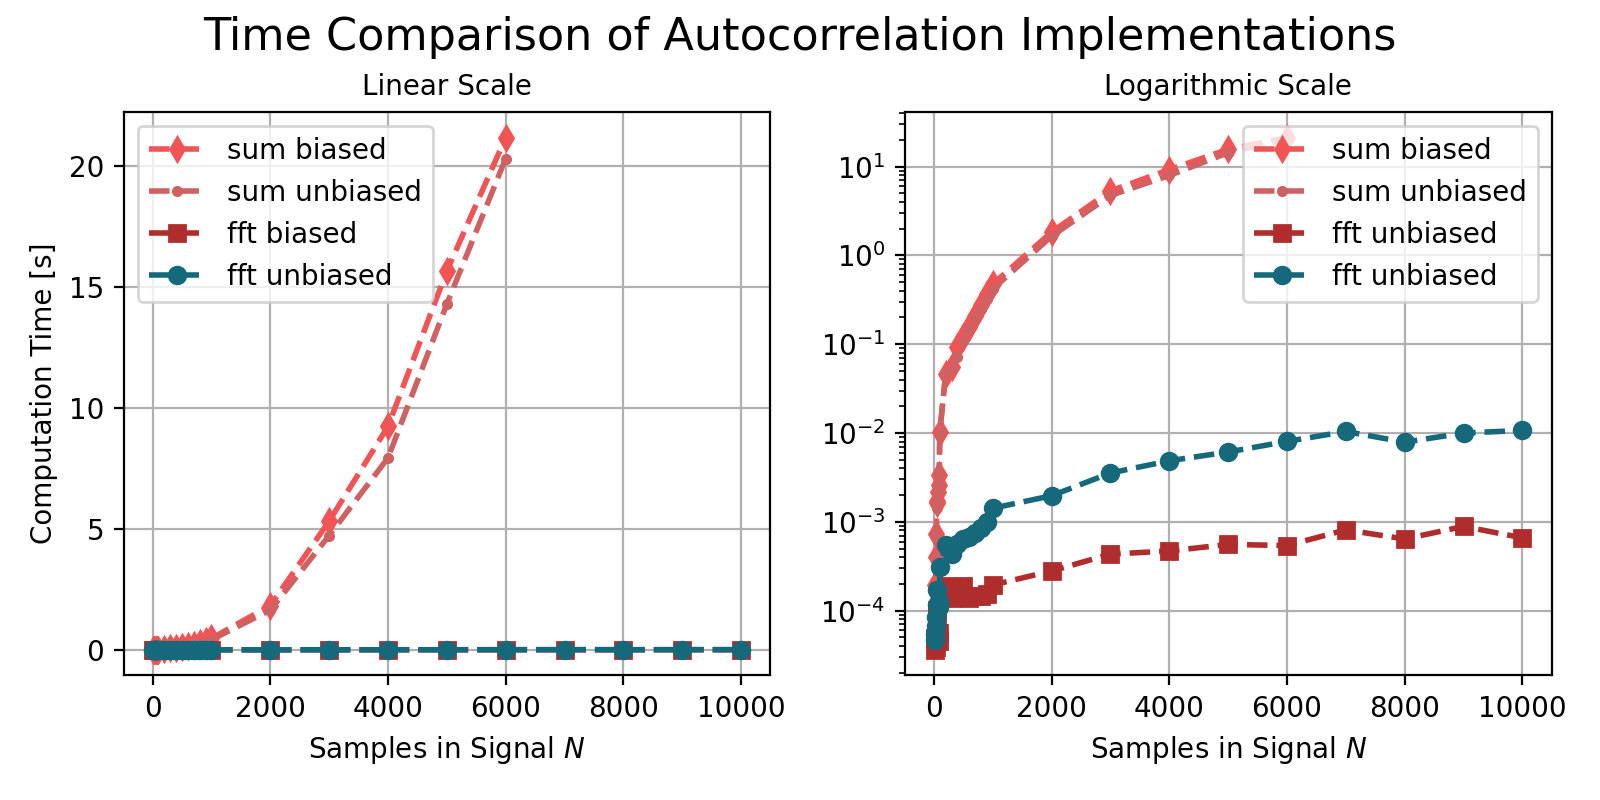
\includegraphics[width=\linewidth]{times}
\vspace{-7mm}
\caption{Time required by each implementation to compute the autocorrelation of an $ N $-sample sinusoidal signal. Note the superiority of the FFT methods.}
\label{fft:fig:times}
\end{figure}


\section{Some Basic Experiments Using Correlation}
The goal of this section is to explore the autocorrelation and cross-correlation of simple signals like sinusoids and normally-distributed random noise before moving to the more complex, real-world signals in \hyperref[fft:s:owls]{Section \ref{fft:s:owls}}.

\subsection{Examining Autocorrelation of Gaussian Noise}
Figure \ref{fft:fig:noise} shows the raw and normalized autocorrelation function of normally distributed random noise with mean $ \mu = 0.5 $ and variance $ \sigma^{2} = 1 $. Characteristically, the autocorrelation is maximum at zero shift and drops rapidly to zero (for the normalized autocorrelation) and to the squared average $ \mu^{2} $ for the raw autocorrelation. 
 
\begin{figure}
\centering
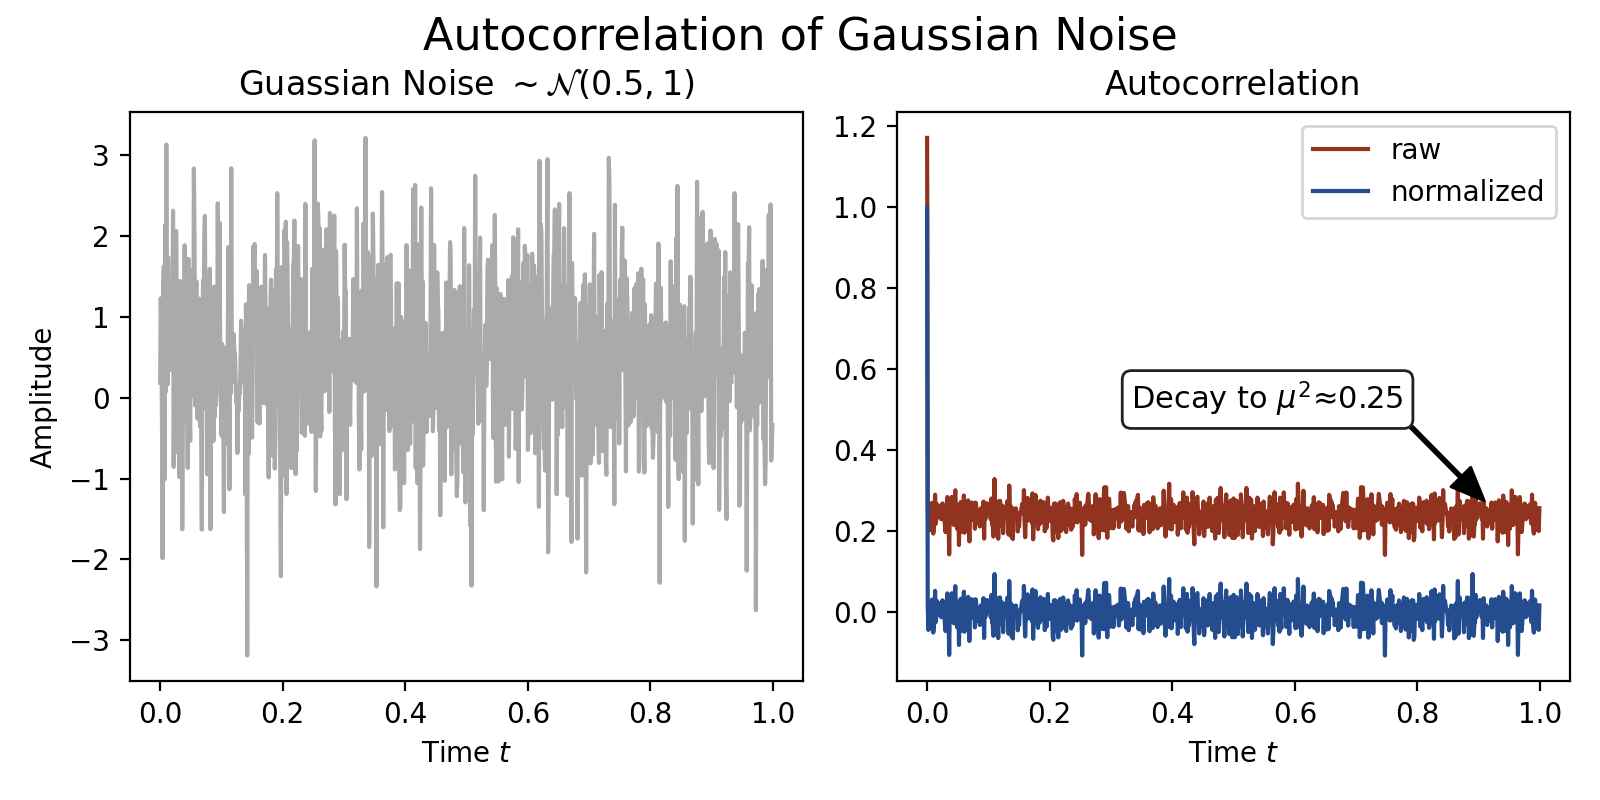
\includegraphics[width=\linewidth]{samples/autocor-noise}
\vspace{-7mm}
\caption{Characteristics of the autocorrelation function of normally distributed random noise. Note the maximum value at zero shift and raw autocorrelation's decay to the mean noise value $ \mu^{2} $ at large shifts. The normalized autocorrelation decays to zero, indicating zero correlation, as expected for noise.}
\label{fft:fig:noise}
\end{figure}



\subsection{Autocorrelation to Detect a Periodic Signal}
Figure \ref{fft:fig:autocor-noisy} shows the autocorrelation of uniformly distributed noise in the range $ [-1, 1] $ superimposed on a sinusoidal function of amplitude with an exponentially decaying envelope. The autocorrelation capably detects the signal's periodicity even as the signal-to-noise ratio exponentially increases. Note that the pure signal is shown only for reference; the autocorrelation is computed using the noisy gray signal.


\begin{figure}
\centering
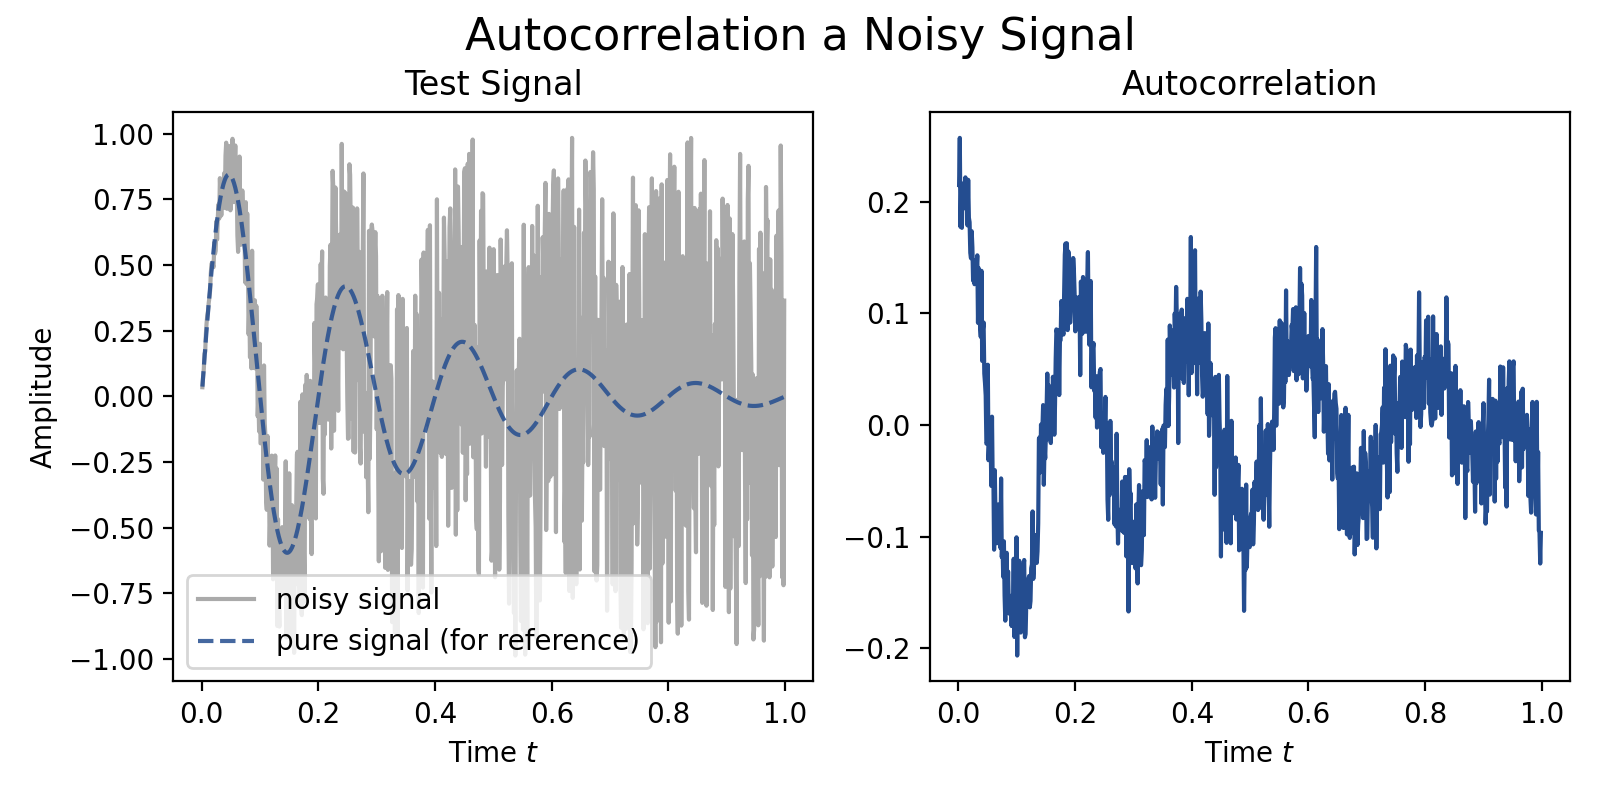
\includegraphics[width=\linewidth]{samples/autocor-noisy}
\vspace{-7mm}
\caption{Autocorrelation of an exponentially decaying sine function (the pure signal is shown in dotted blue for reference) masked with uniformly distributed noise. The autocorrelation detects periodicity even at a large SNR, when doing so visually would be difficult.}
\label{fft:fig:autocor-noisy}
\end{figure}



\subsection{Cross-Correlation to Detect a Periodic Signal}
In this example, I first superimposed a short, weak sine wave on normally distributed random noise with mean $ \mu = 0 $ and variance $ \sigma^{2} = 1 $, shown in Figure \ref{fft:fig:crosscor-noisy}. I then used the pure sine signal as a cross-correlation ``probe'' to detect the onset of the weak periodic signal within the noisy signal. Note that, as before, the pure probe signal is shown only for reference; the autocorrelation is calculated on the noisy gray signal. I found the results quite impressive---if the probe signal were not retrospectively highlighted for reference, visually identifying its position within the noisy signal seems hopeless, but the cross-correlation function does so definitively. I used a similar approach in \hyperref[fft:ss:bubo-cross-cor]{Subsection \ref{fft:ss:bubo-cross-cor}} to detect owl calls.

\begin{figure}
\centering
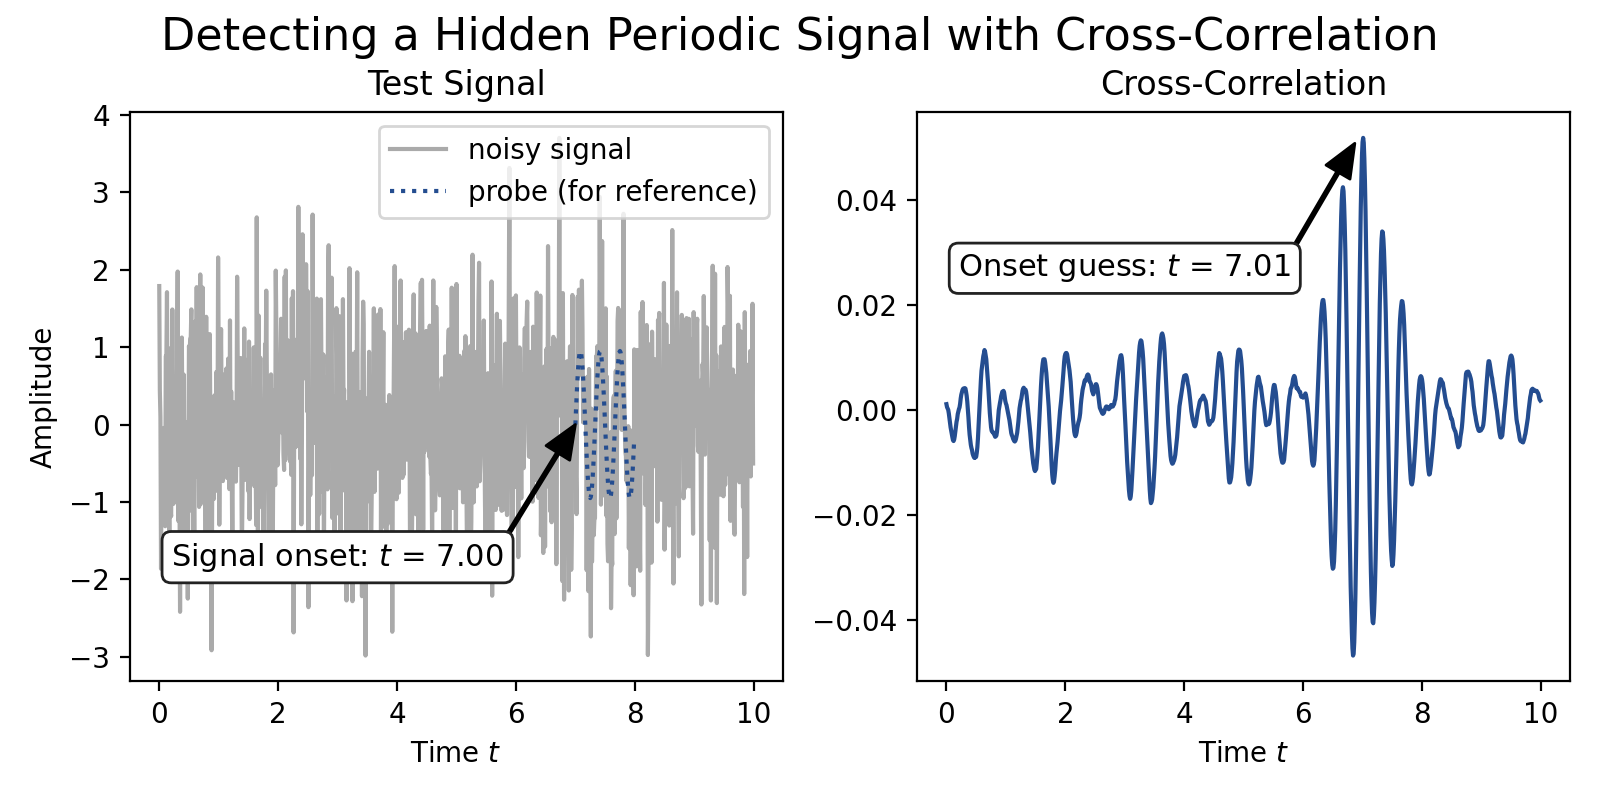
\includegraphics[width=\linewidth]{samples/crosscor-noisy}
\vspace{-7mm}
\caption{Using cross-correlation to detect the onset of a weak periodic signal within normally distributed random noise $ \sim \mathcal{N}(0, 1) $. The signal onset corresponds the the cross-correlation's maximum. The correct position of the ``probe'' signal is shown in dashed blue for reference. }
\label{fft:fig:crosscor-noisy}
\end{figure}


\section{Identifying Eurasian Eagle Owls with Correlation} \label{fft:s:owls}
First, some background: we are given the ``clean'', noiseless calls of two different Eurasian eagle owls in \SI{44100}{\hertz}, single-channel \texttt{wav} format, along with four records of the same two owls in noisy natural environments. The goal is to detect which owl in the noisy recordings is which based on the ``clean'' reference calls. For orientation, a quick description of each recording follows below, while Figure \ref{fft:fig:bubo-waveforms} shows the corresponding waveforms in the time domain. 
\begin{itemize}
	\item \texttt{bubomono.wav} and \texttt{bubo2mono.wav}: 5-second clips containing the first and second owl's call, respectively. The calls themselves last from about \SIrange{0.5}{1.0}{\second}; the rest of each file is faint background noise. 
	
	\item \texttt{bubo1-short.wav} and \texttt{bubo2-short.wav}: \SI{0.5}{\second} trimmed versions of \texttt{bubomono.wav} and \texttt{bubo2-short.wav} containing only the owl calls.
	
	\item \texttt{mix.wav}: Light background noise including crickets and the sound of a person walking through brush and dry leaves. The owl call is heard clearly.
	
	\item \texttt{mix1.wav}: Moderate background noise including a burbling creek and cricket song. The owl call is heard well, but not as clearly as in \texttt{mix.wav}.
	
	\item \texttt{mix2.wav}: Loud background noise including a running river and gentle crickets. The owl call is faint.
	
	\item \texttt{mix22.wav}: Dominant background noise from a running river. The owl call is hardly audible.
	
\end{itemize}
Each \texttt{mix} file is a 5-second recording with the owl call near the \SI{0.5}{\second} mark.


\begin{figure}[htb!]
	\centering
	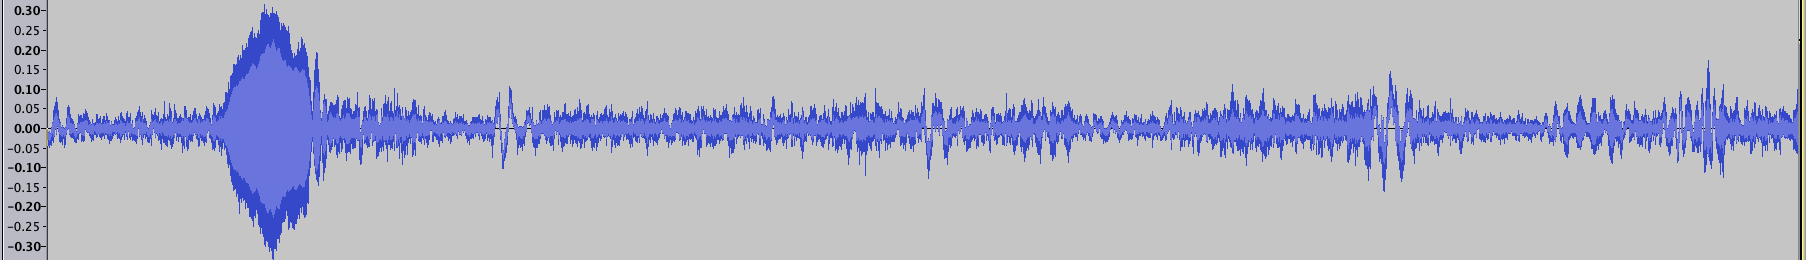
\includegraphics[width=\linewidth]{waveforms/mix}\vfill  
	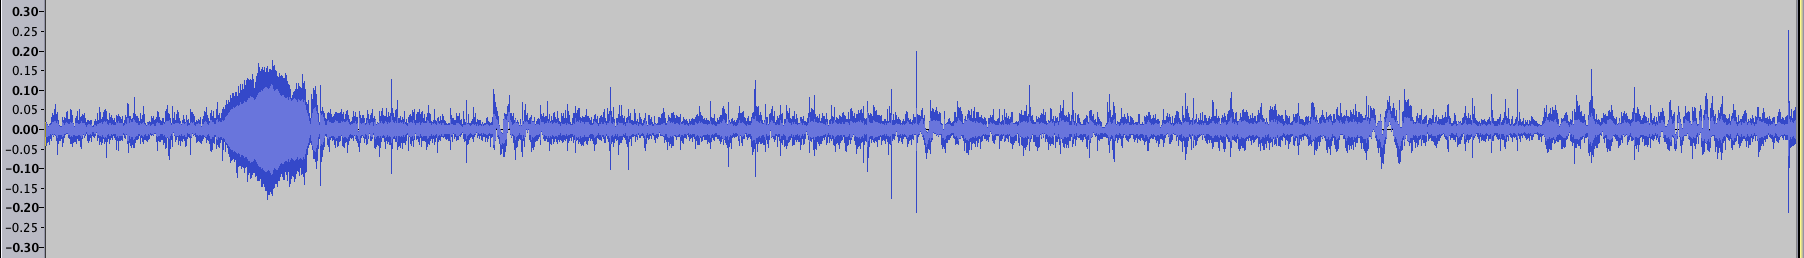
\includegraphics[width=\linewidth]{waveforms/mix1}\vfill  
	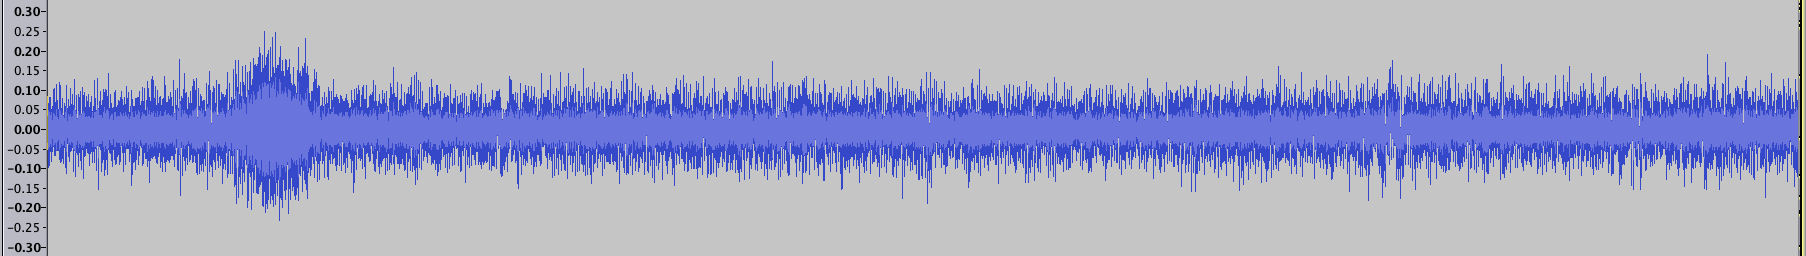
\includegraphics[width=\linewidth]{waveforms/mix2}\vfill
	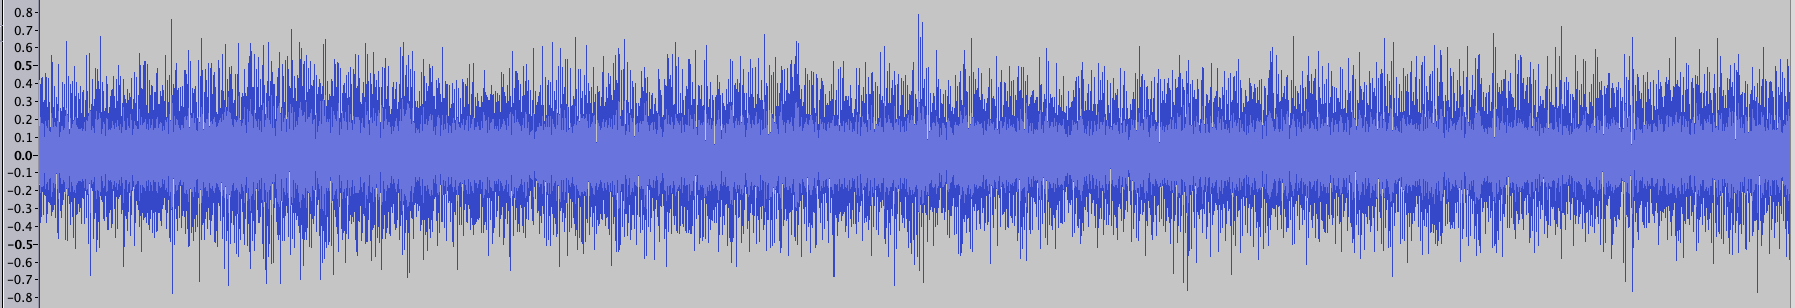
\includegraphics[width=\linewidth]{waveforms/mix22}\vfill    
	\caption{Time-domain waveforms, in order from top to bottom, of the recordings \texttt{mix}, \texttt{mix1}, \texttt{mix2}, \texttt{mix22}. Note how the owl call---the short peak near the beginning of each clip---is progressively dominated by background noise in successive recordings.}
	\label{fft:fig:bubo-waveforms}
\end{figure}


\subsection{Cross-Correlation Analysis} \label{fft:ss:bubo-cross-cor}
This is the first of two approaches to identifying the owl in each noisy signal. The premise is simple: I used the ``clean'' reference recordings \texttt{bubo1.wav} and \texttt{bubo2.wav} as cross-correltion ``probes'' to analyze each \texttt{mix} recording. The reference recording producing a stronger cross-correlation response would identify the owl in each noisy signal. The method worked impressively---see Figures \ref{fft:fig:bubo-crosscor1} and \ref{fft:fig:bubo-crosscor2} for results. For perspective, in the noisiest recording \texttt{mix22}, the listener is hard-pressed to make out a hoot in the first place, let alone identify the correct owl---just look at the last waveform in Figure \ref{fft:fig:bubo-waveforms}, which appears to be pure noise. But the cross-correlation in Figure \ref{fft:fig:bubo-crosscor2} performs the identification capably. I was impressed, to say the least!



\begin{figure}[htb!]
	\centering
	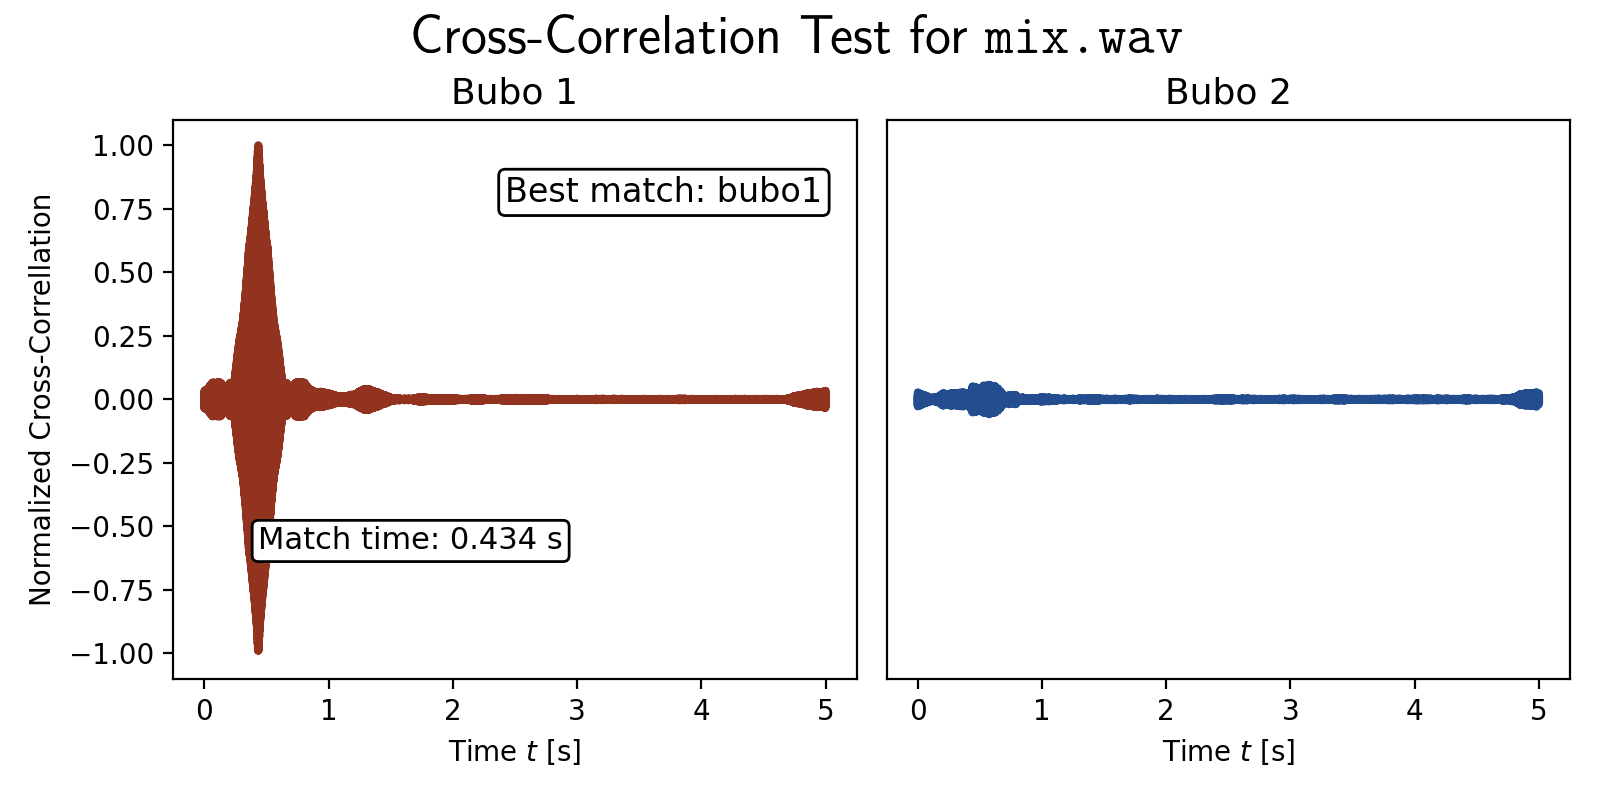
\includegraphics[width=\linewidth]{cross-cor/mix-crosscor}\vfill  
	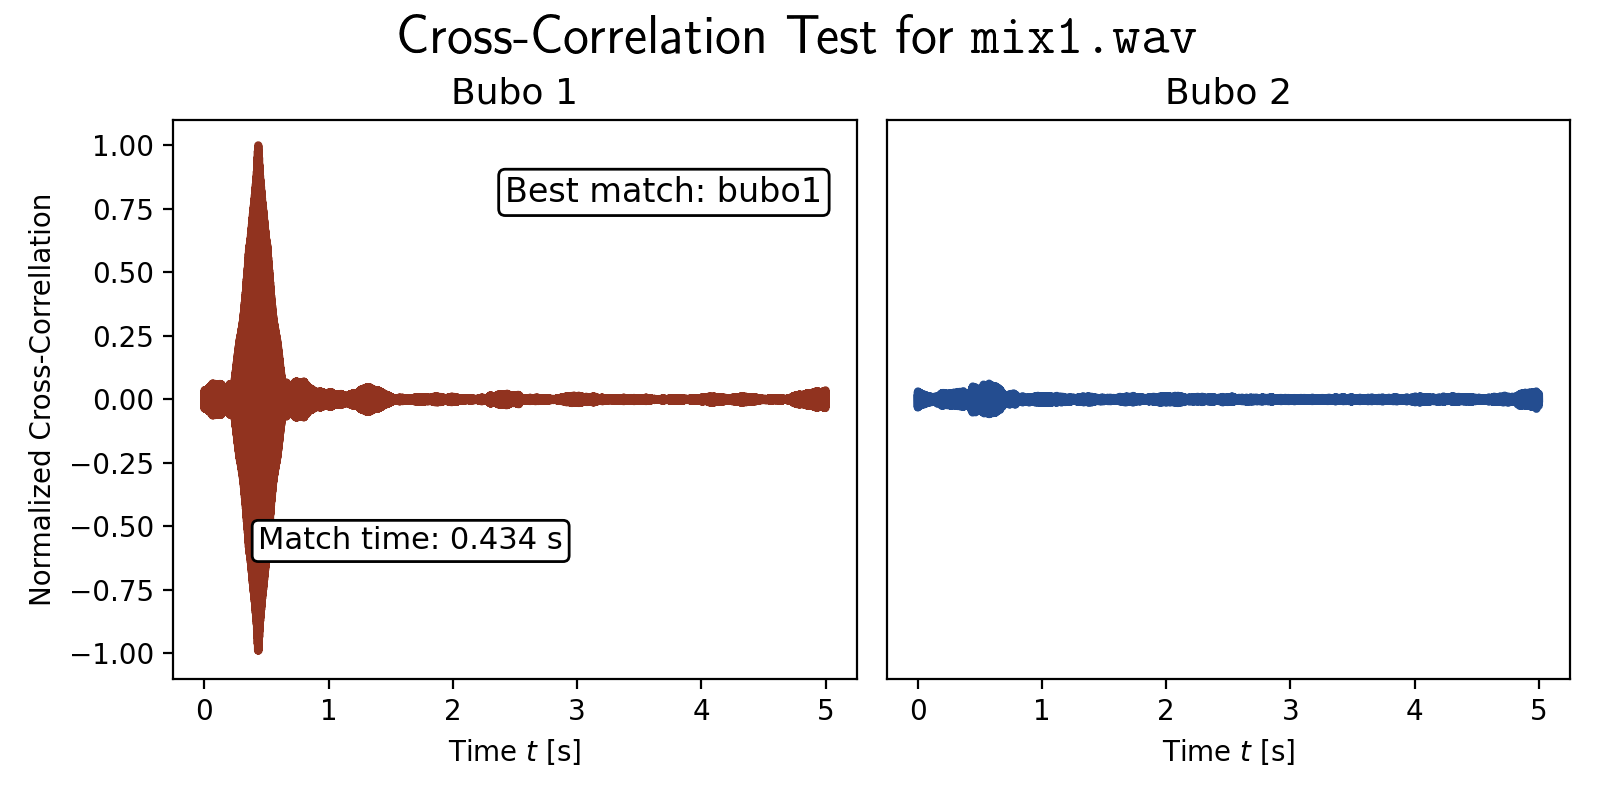
\includegraphics[width=\linewidth]{cross-cor/mix1-crosscor}\vfill  
	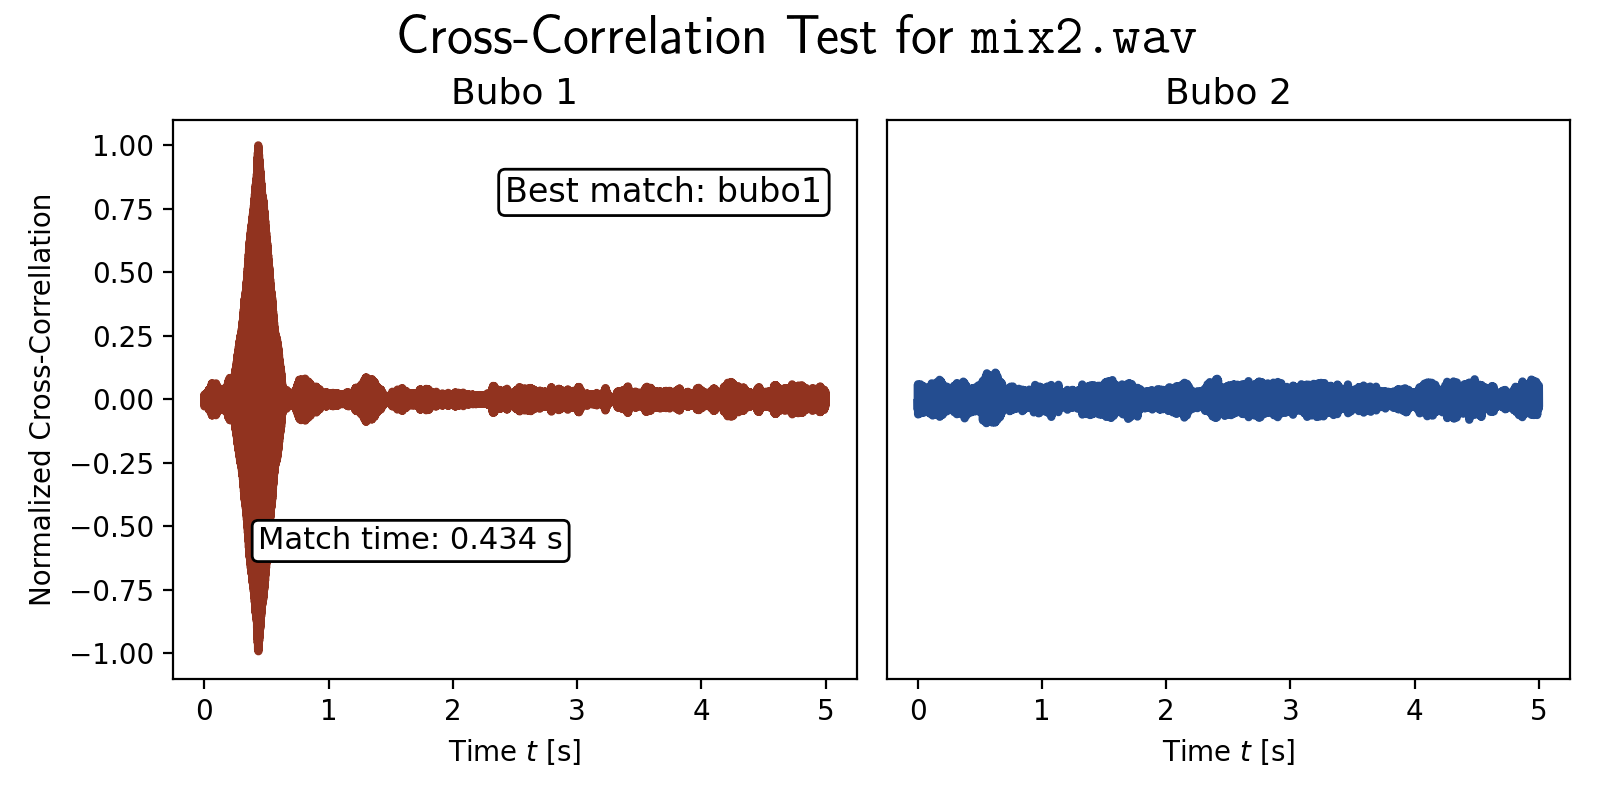
\includegraphics[width=\linewidth]{cross-cor/mix2-crosscor}\vfill  
	\caption{Identifying the owl in the noisy recordings \texttt{mix}, \texttt{mix1} and \texttt{mix2} via cross-correlation with the clean reference calls.}
	\label{fft:fig:bubo-crosscor1}
\end{figure}

\begin{figure}[htb!]
	\centering
	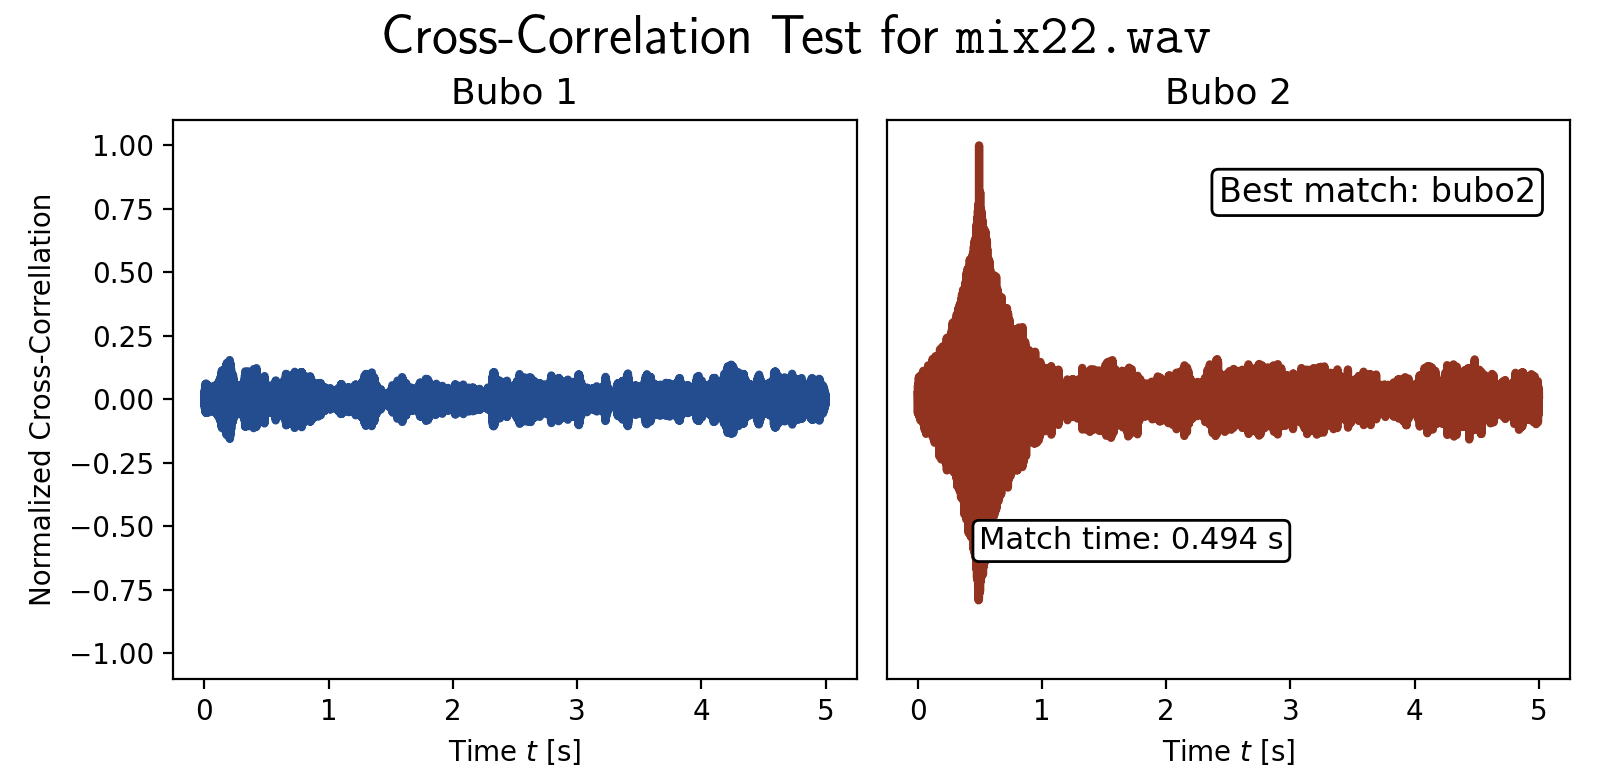
\includegraphics[width=\linewidth]{cross-cor/mix22-crosscor}\vfill  
	\caption{Identifying the owl \texttt{bubo2} in the noisy recording \texttt{mix22} using cross-correlation with the clean reference calls.}
	\label{fft:fig:bubo-crosscor2}
\end{figure}





\subsection{Spectral Analysis}
This approach works by identifying the characteristic frequency of each owl from the clean reference calls and then searching for the presence of the characteristic frequency in the spectrum of each noisy recording. 

\subsubsection{Spectrum of Pure Owl Calls}
First, I plotted the spectrum of the reference signals \texttt{bubo1-short.wav} and \texttt{bubo2-short.wav}. Each owl call displays a clear and distinct fundamental frequency---\SI{380}{\hertz} for \texttt{bubo1} and \SI{335}{\hertz} for \texttt{bubo2}---along with higher harmonics at integer multiples of the fundamental. Figure \ref{fft:fig:probe-spectra} shows both spectra in linear and logarithmic scale; the latter is useful when identifying the higher harmonics.


\begin{figure}[htb!]
	\centering
	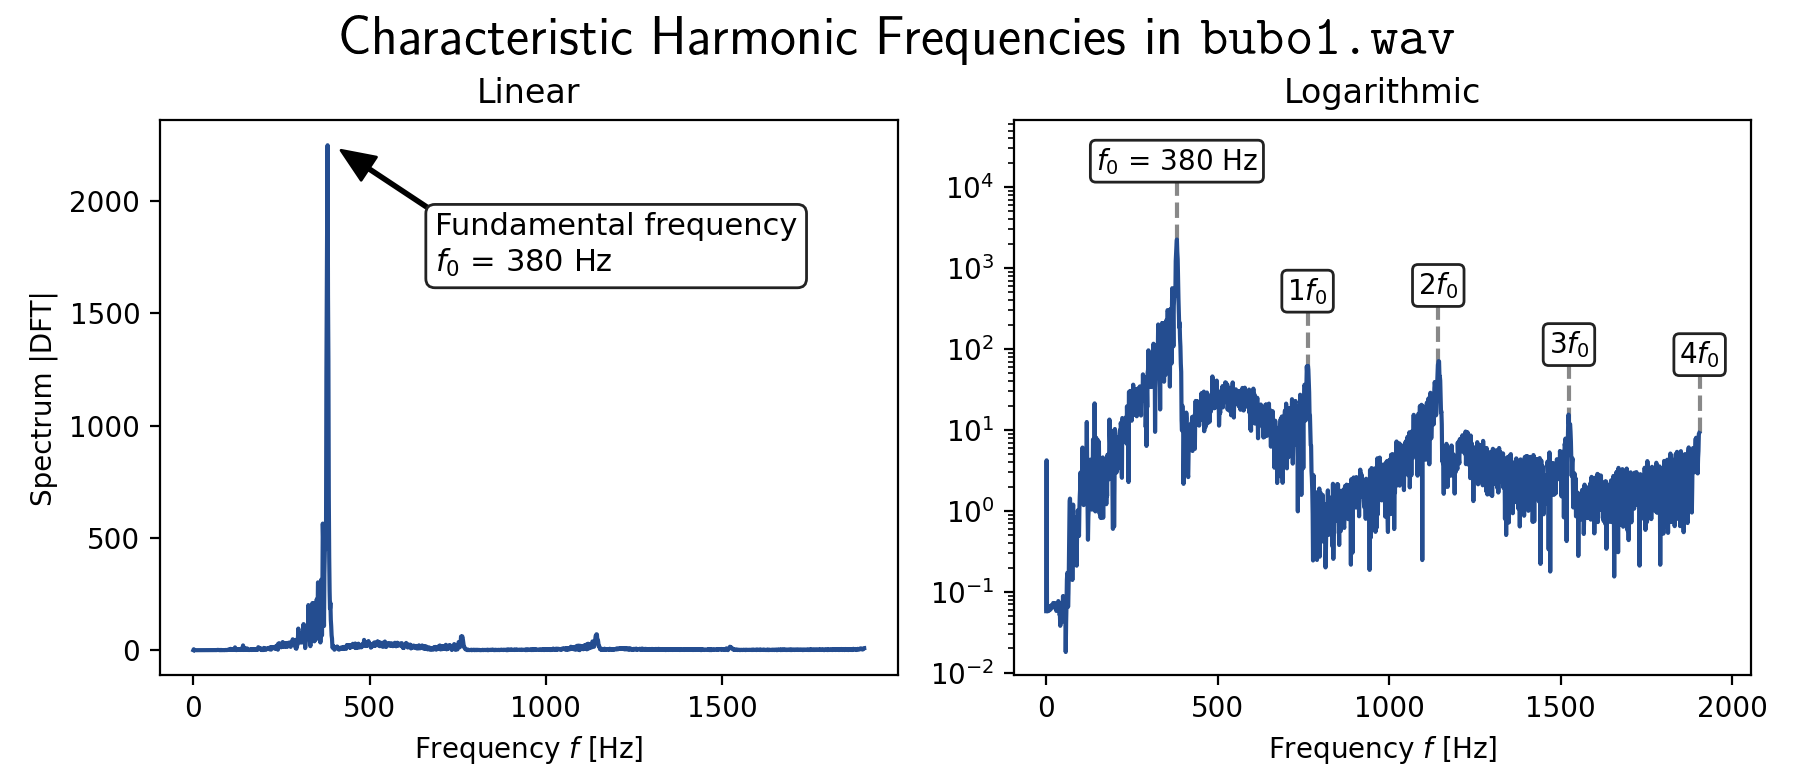
\includegraphics[width=\linewidth]{spectra/bubo1-spectrum}\vfill  
	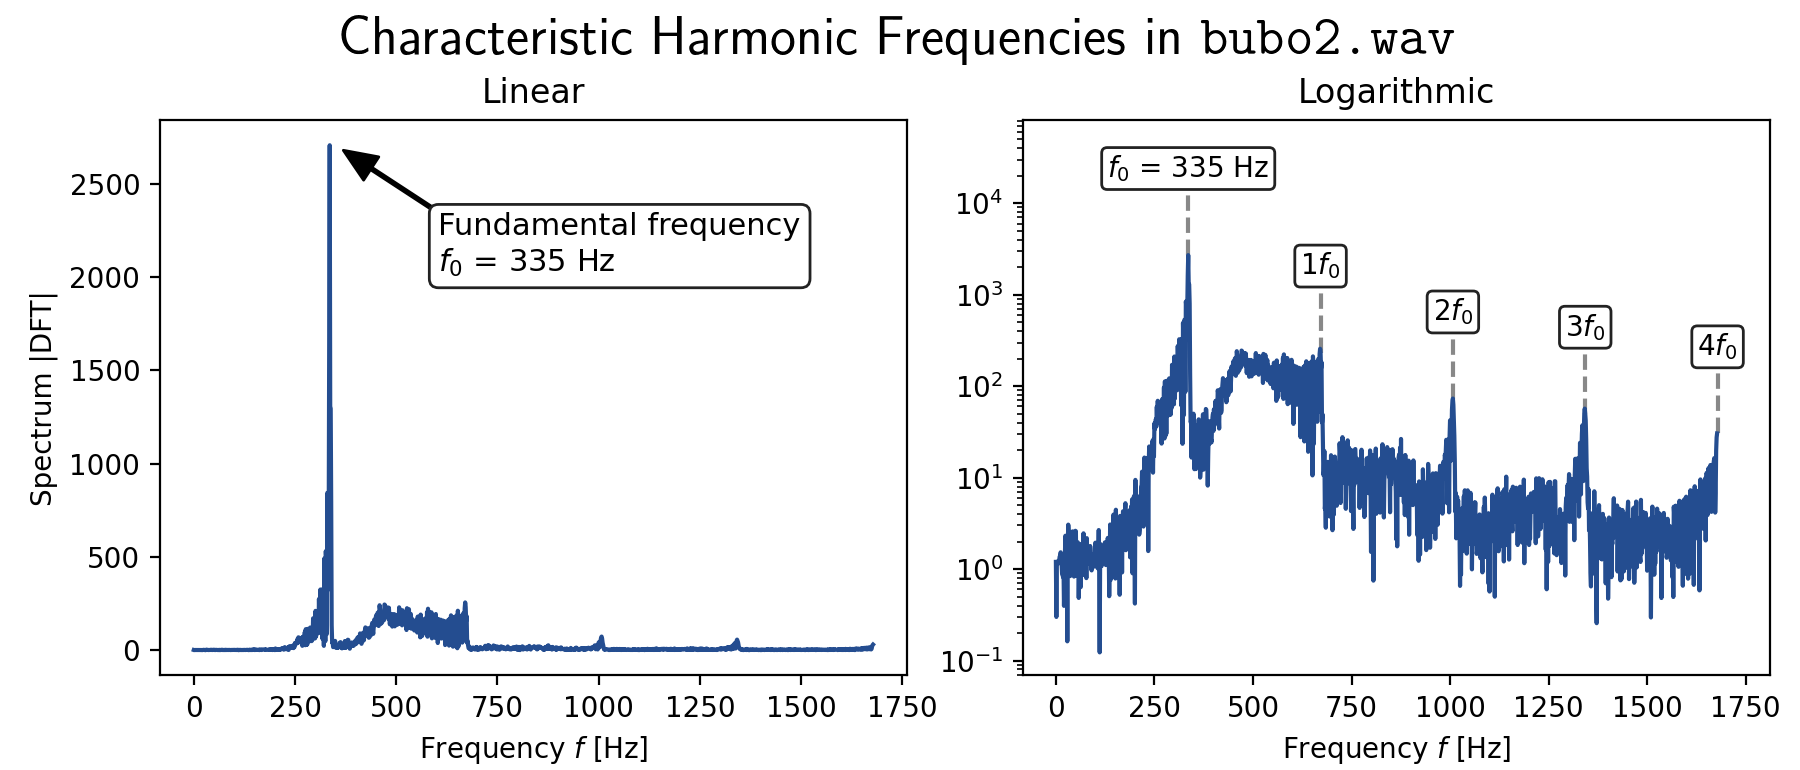
\includegraphics[width=\linewidth]{spectra/bubo2-spectrum}\vfill  
	\caption{Both owl calls display clear and distinct fundamental frequencies---either \SI{380}{\hertz} for \texttt{bubo1} or \SI{335}{\hertz} for \texttt{bubo2}. These frequencies are used later as ``acoustic fingerprints'' to identify the owls in noisy recordings.}
	\label{fft:fig:probe-spectra}
\end{figure}
 

\subsubsection{Analysis of Signal and Autocorrelation Spectrum}
The premise of this method is straightforward: compute the spectrum of each noisy signal and search for the presence of a fundamental frequency from Figure \ref{fft:fig:probe-spectra} that would uniquely identify the owl, either \SI{380}{\hertz} for \texttt{bubo1} or \SI{335}{\hertz} for \texttt{bubo2}. There is a slight caveat---I found used the spectra of both the raw signal and the signal's autocorrelation function. 

Why use the autocorrelation's spectrum? My thinking was: each noisy signal contains a characteristic owl frequency, which should be picked up by the autocorrelation function (the autocorrelation of a periodic signal is periodic with the same period), with a slight bonus---the autocorrelation should remove random noise from each noisy signal (see e.g. the derivation in Equation \ref{fft:eq:autocor-noise-removal}). Figure \ref{fft:fig:autocor-periodic} shows how the autocorrelation of the noisy signal \texttt{mix1.wav} is indeed periodic; the other \texttt{mix} files all display periodicity, and I left them out to avoid over-cluttering the report with figures.


\begin{figure}[htb!]
	\centering
	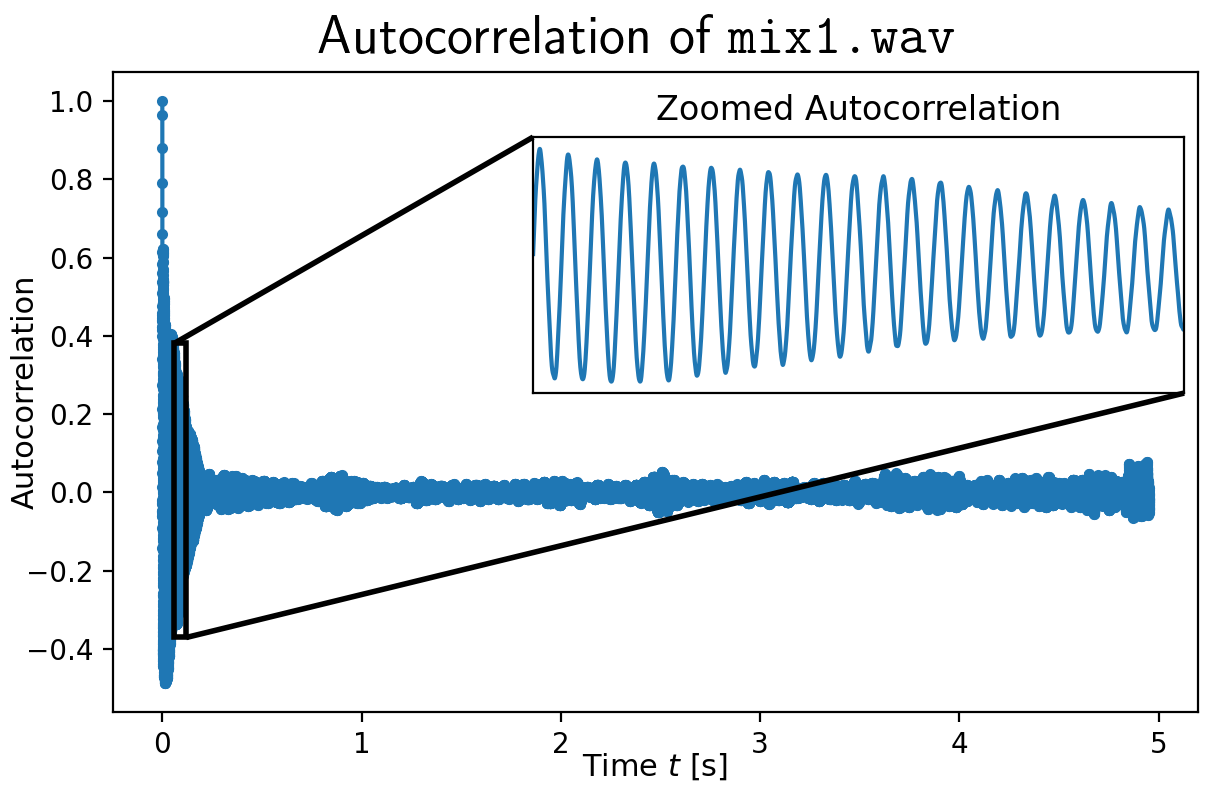
\includegraphics[width=\linewidth]{autocor/mix1-autocor}  
	\caption{The autocorrelation function of \texttt{mix1.wav}. The zoomed portion is intended to show how the autocorrelation function is periodic, presumably at the characteristic frequency of the owl call, which forms the basis of the spectral analysis in Figures \ref{fft:fig:mix-spectra1} and \ref{fft:fig:mix-spectra2}.}
	\label{fft:fig:autocor-periodic}
\end{figure}
\begin{figure}[htb!]
	\centering
	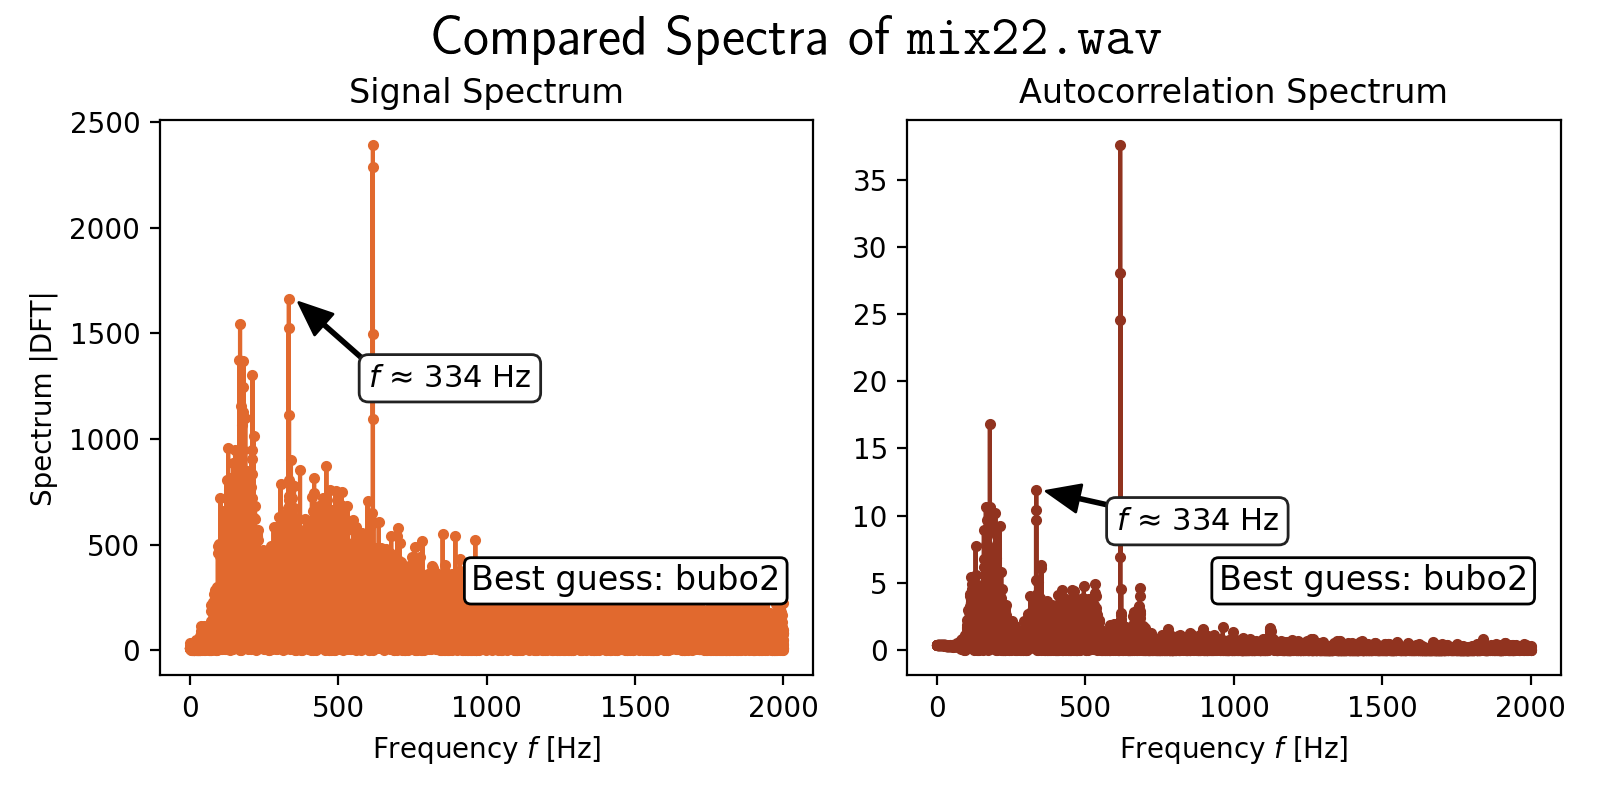
\includegraphics[width=\linewidth]{spectra/mix22-compared-spectra}  
	\caption{The spectra of the raw noisy signal and the signal's autocorrelation function both display the \SI{335}{\hertz} characteristic frequency of \texttt{bubo2} in the recording \texttt{mix22}.}
	\label{fft:fig:mix-spectra2}
\end{figure}


The spectral approach appears to correctly identify the owl in each recording, although the results are not as definitive as when using cross-correlation detection. Note that the autocorrelation's spectrum is indeed less noisy than the raw signal's spectrum, but only up to a constant factor of order $ 1 $. I was impressed by both spectra picking up nearly identical frequencies, indicating that the autocorrelation function successfully preserves the dominant frequencies in the noisy signal.


\begin{figure}[htb!]
	\centering
	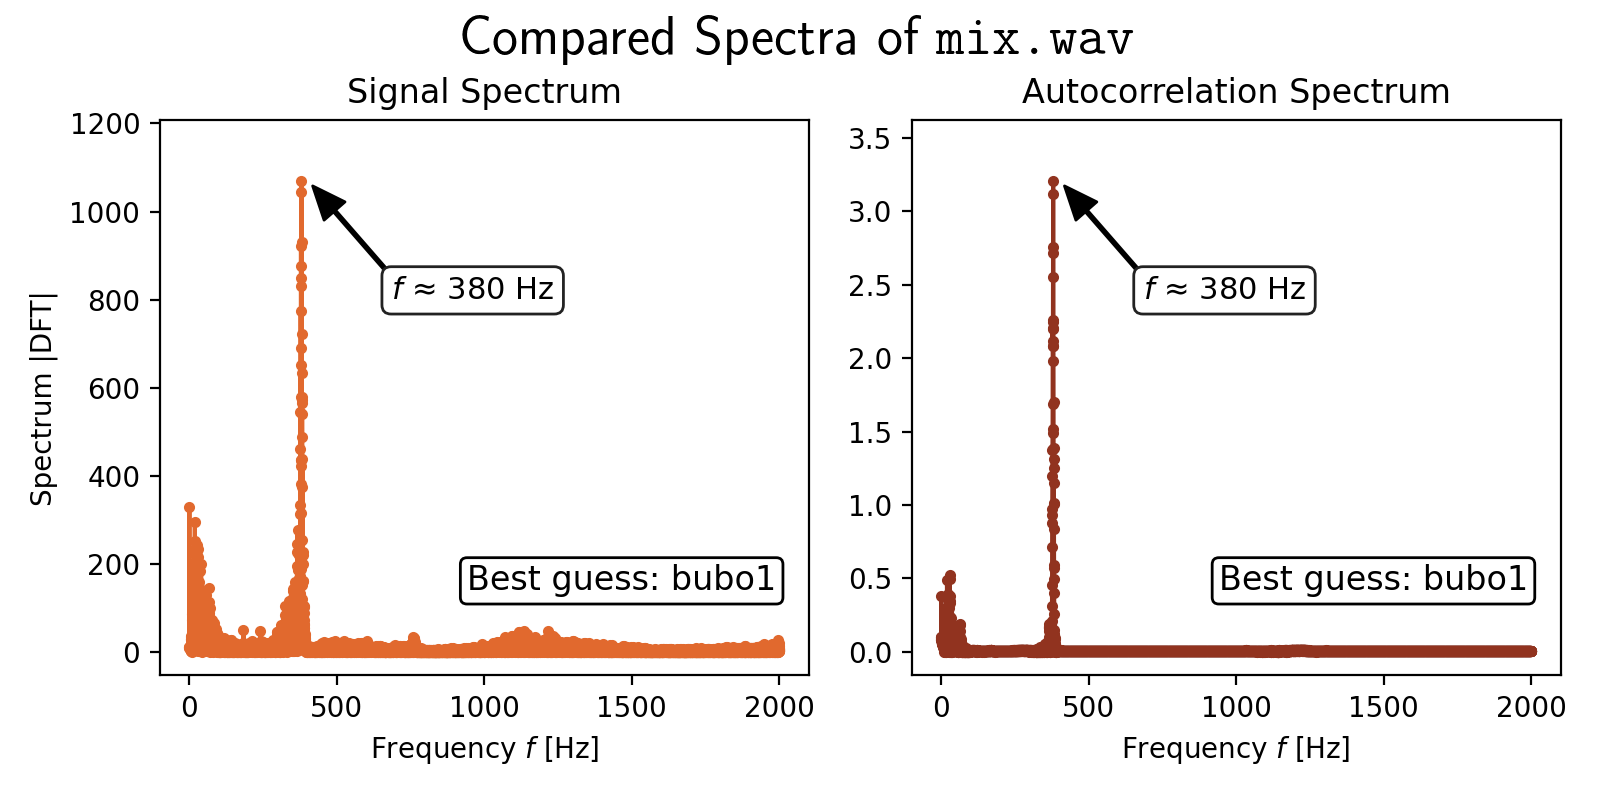
\includegraphics[width=\linewidth]{spectra/mix-compared-spectra}\vfill  
	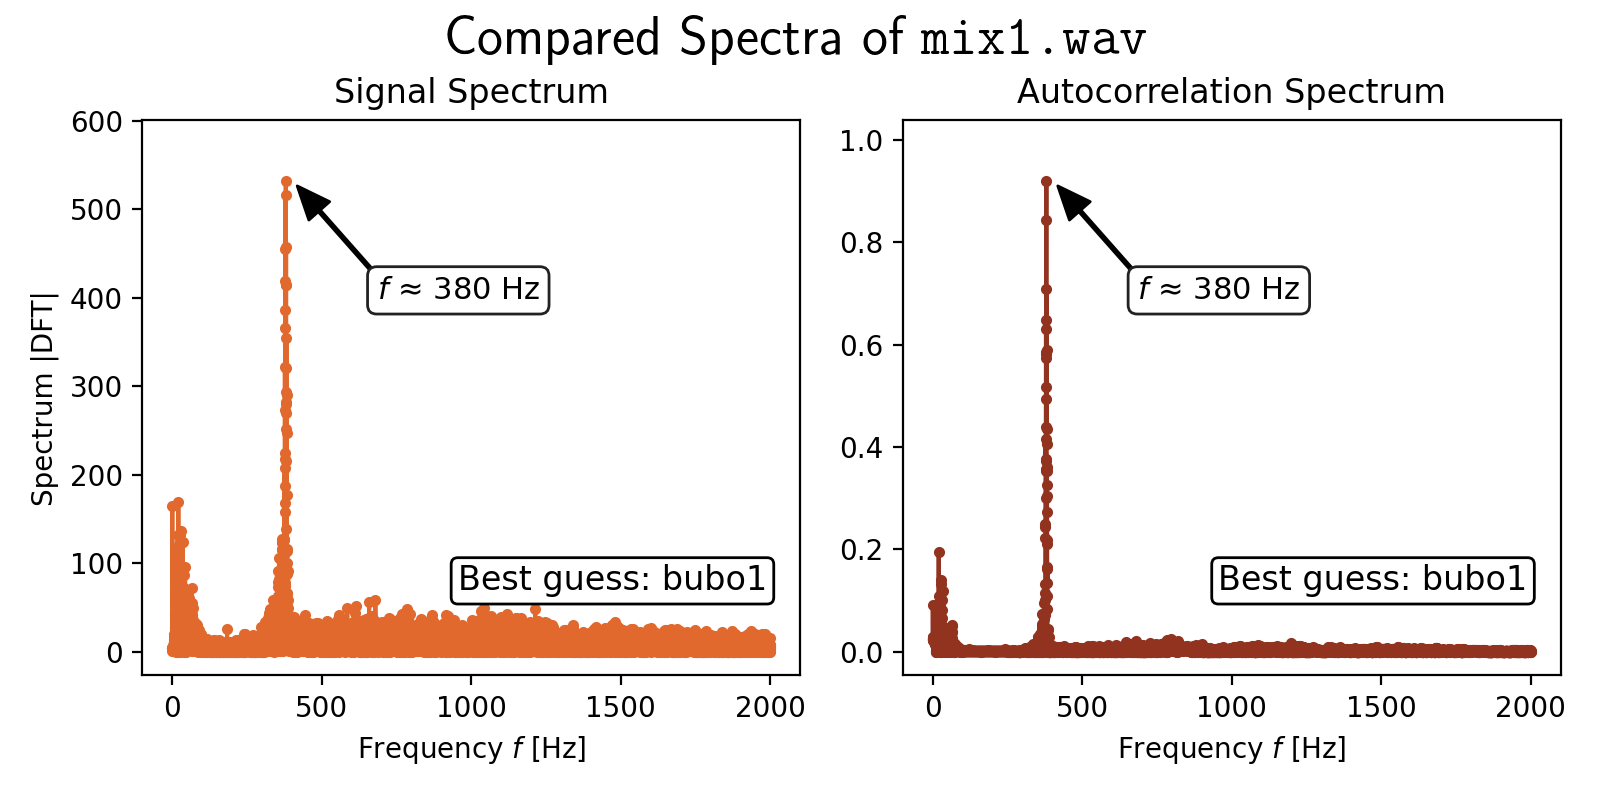
\includegraphics[width=\linewidth]{spectra/mix1-compared-spectra}\vfill  
	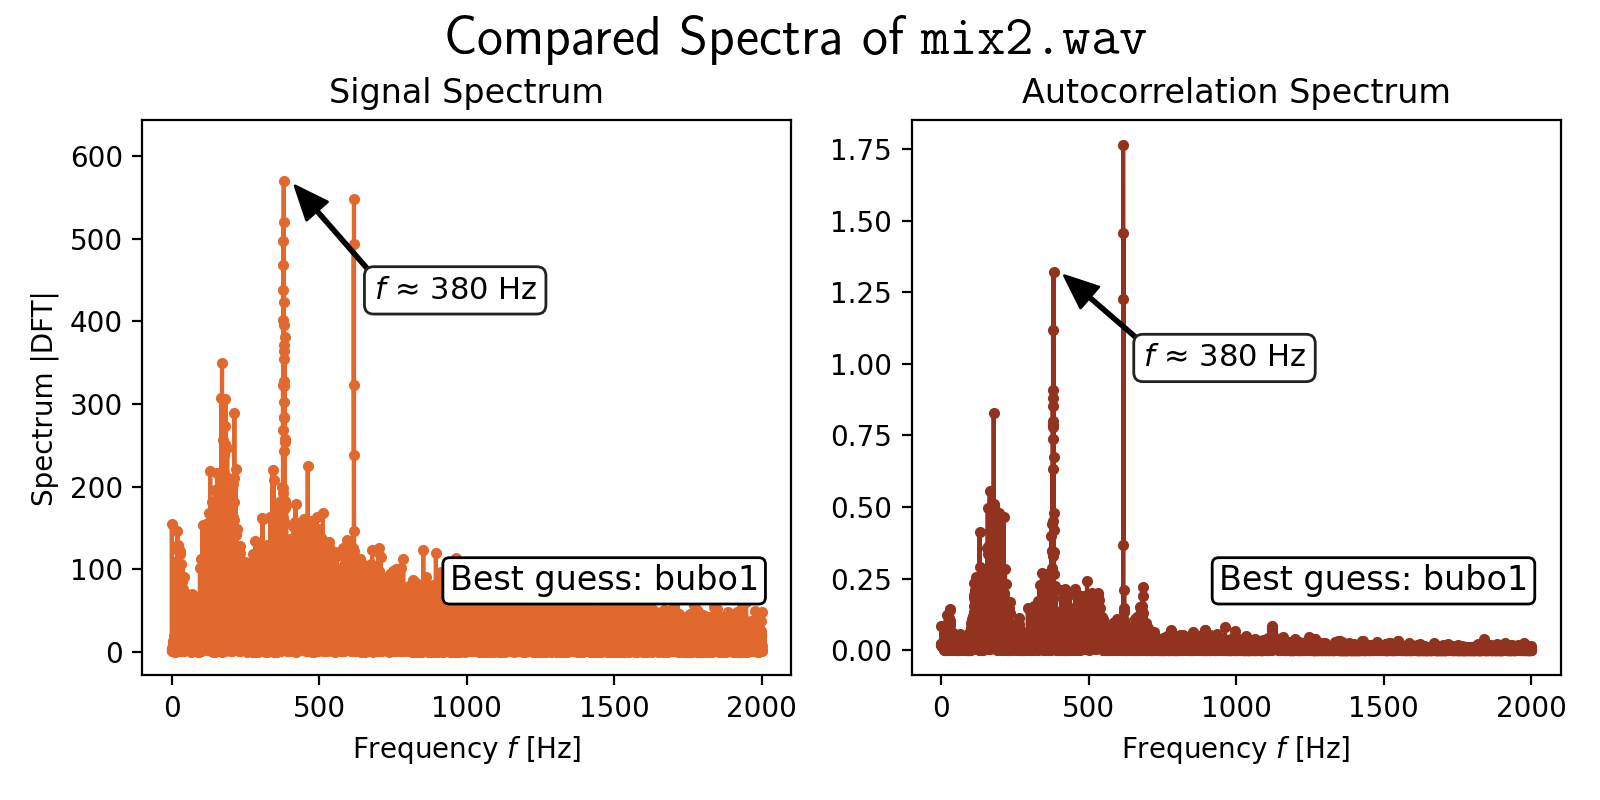
\includegraphics[width=\linewidth]{spectra/mix2-compared-spectra}\vfill  
	\caption{The spectra of the raw noisy signal and the signal's autocorrelation function both display the characteristic frequency \SI{380}{\hertz} characteristic frequency of \texttt{bubo1} in the recordings \texttt{mix}, \texttt{mix1} and \texttt{mix2}.}
	\label{fft:fig:mix-spectra1}
\end{figure}




\subsection{Quick Summary of Results}
Table \ref{fft:table:results} summarizes the identification results for each of the three methods used in the report. All of methods agree on their identification for each noisy file. 
\begin{table}[h]
\centering
\begin{tabular}{c|cccc}
    Method & \texttt{mix} & \texttt{mix1} & \texttt{mix2} & \texttt{mix22} \\
    \hline
    Cross-Correlation & \texttt{bubo1} & \texttt{bubo1} & \texttt{bubo1} & \texttt{bubo2}\\
    Signal Spectrum & \texttt{bubo1} & \texttt{bubo1} & \texttt{bubo1} & \texttt{bubo2}\\
    Autocorrelation Spectrum & \texttt{bubo1} & \texttt{bubo1} & \texttt{bubo1} & \texttt{bubo2}
\end{tabular}
\label{fft:table:results}

\end{table}

\section{Extra: Extracting Guitar Notes from a Noisy Background}
As an extra, I recorded (in \SI{44100}{\hertz} sample rate, single-channel, \texttt{wav} format) individual reference samples of three notes played on an acoustic guitar---the \texttt{E3}, \texttt{A3} and \texttt{G4} notes to use as reference ``probe signals'', and then recorded the same notes played in the sequence 
\begin{center}
	\texttt{E3} \qquad \texttt{G4} \qquad  \texttt{A3}
\end{center}
with the notes spaced at roughly one second intervals. I'll refer to this recording at \texttt{sequence-clean.wav}.\footnote{As a side note, I intentionally played the notes as string harmonics at the 12th fret to produce a weaker signal (and thus push the limits of the correlation detection), but that is a non-essential musical detail.} 

Next, inspired by the \texttt{bubo} recordings, I superimposed various nature sounds (songbirds, ocean waves crashing on a beach, and a running river) on the clean signal to generate the noisy files \texttt{sequence-waves.wav}, \texttt{sequence-birds-river.wav}, and \texttt{sequence-birds-waves.wav}.\footnote{The samples are included, along with the usual source code, in the \texttt{zip} file accompanying the report.} To push the limits of correlation detection, I increased the noise amplitude well above the actual signal amplitude (at least on par with the noisiest owl recording \texttt{mix22.wav})---in \texttt{sequence-birds-waves}, for example the \texttt{E} and \texttt{A} notes are hardly audible.

I then performed an analogous cross-correlation analysis to those shown and discussed in Figure \ref{fft:fig:crosscor-noisy} and \hyperref[fft:ss:bubo-cross-cor]{Subsection \ref{fft:ss:bubo-cross-cor}}; the goal was to detect the onset of each note in the noisy signal. Figures \ref{fft:fig:G4-crosscor} through \ref{fft:fig:A3-crosscor} show the results. The method works well, generally detecting the note's onset time to withing a few milliseconds (the reference value was determined from \texttt{sequence-clean.wav} in the audio editing and waveform analysis program \texttt{Audacity}). Worth noting, however, is that the method failed for the first \texttt{E3} note in the recordings \texttt{sequence-waves.wav} and \texttt{sequence-birds-waves.wav}. Whether the failure is a fault of the cross-correlation method in principle or my overzealous attempts to push the method to its limit by making the \texttt{E3} note excessively faint relative to the dominating background noise is up to debate---I encourage the reader to give the recordings \texttt{sequence-birds-waves.wav} and \texttt{sequence-waves.wav} a listen and decide for him or herself. 


\begin{figure}[htb!]
	\centering
	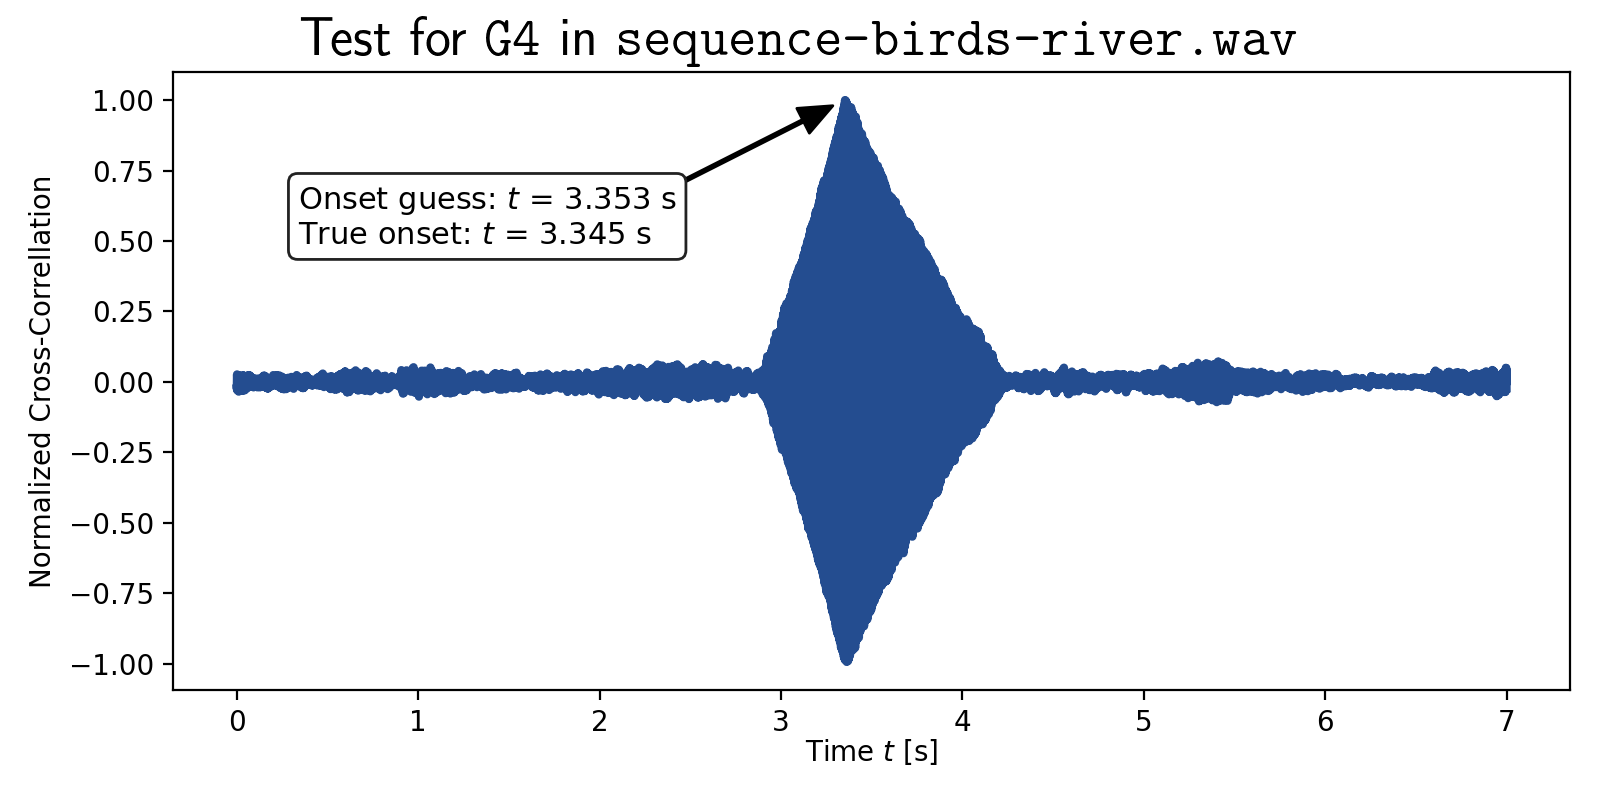
\includegraphics[width=\linewidth]{cross-cor/G4-sequence-birds-river}\vfill  
	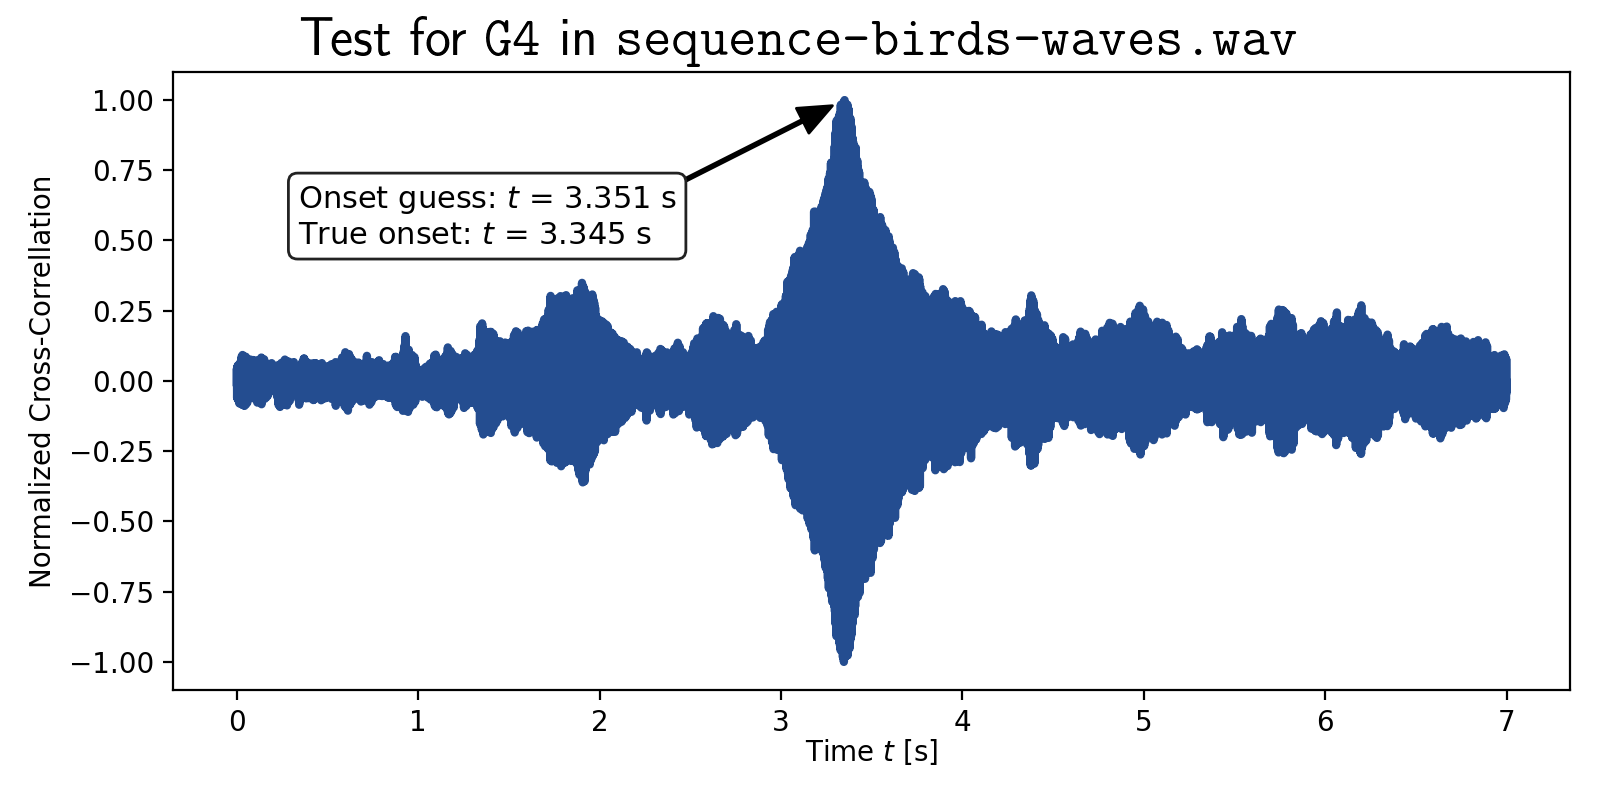
\includegraphics[width=\linewidth]{cross-cor/G4-sequence-birds-waves}\vfill  
	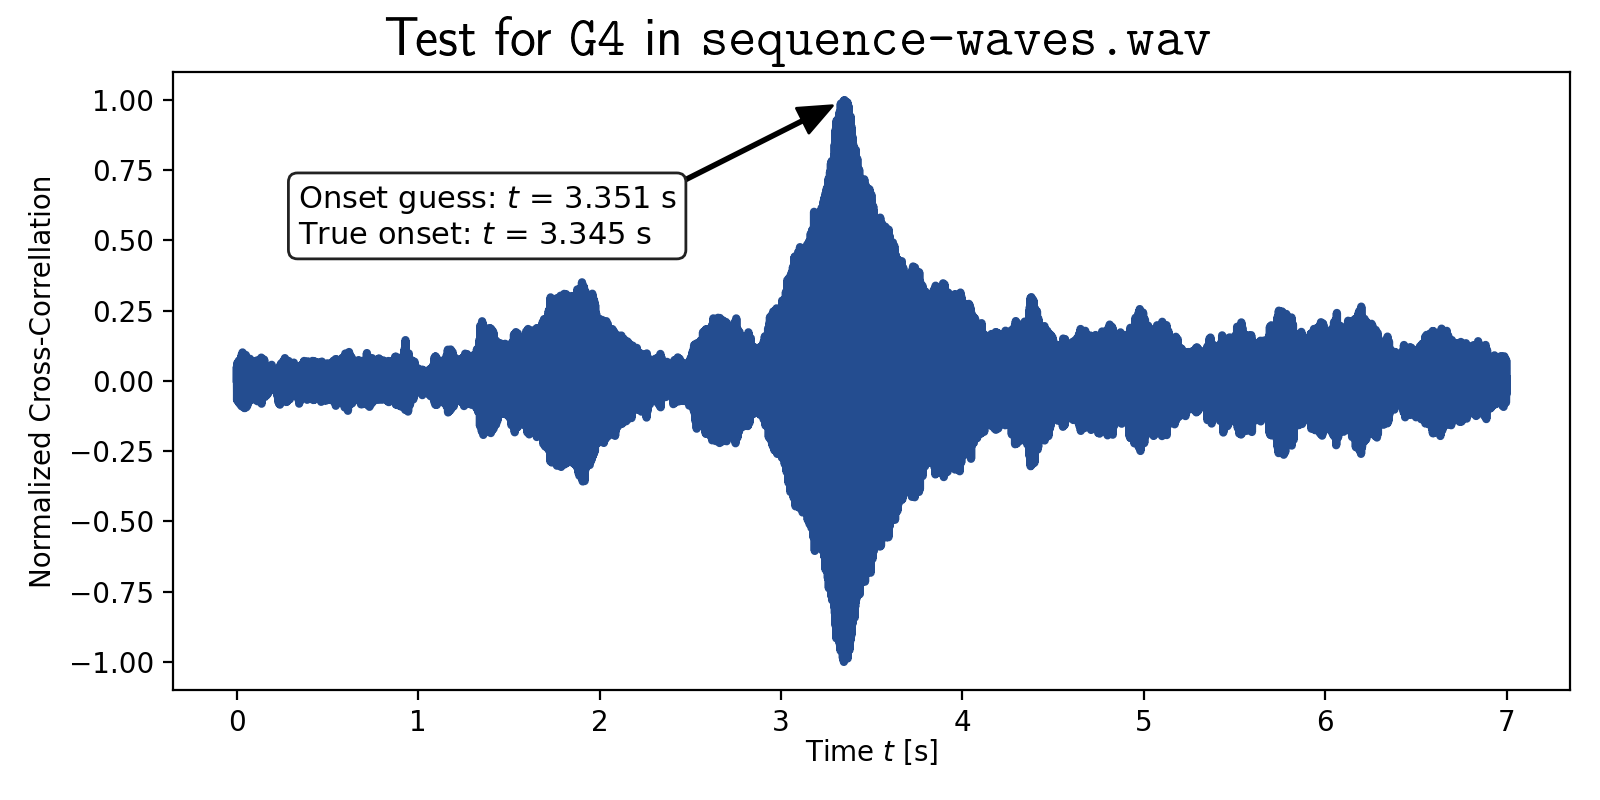
\includegraphics[width=\linewidth]{cross-cor/G4-sequence-waves}\vfill  
	\caption{Using cross-correlation to detect the onset of a faint \texttt{G4} note in a noisy background.}
	\label{fft:fig:G4-crosscor}
\end{figure}

\begin{figure}[htb!]
	\centering
	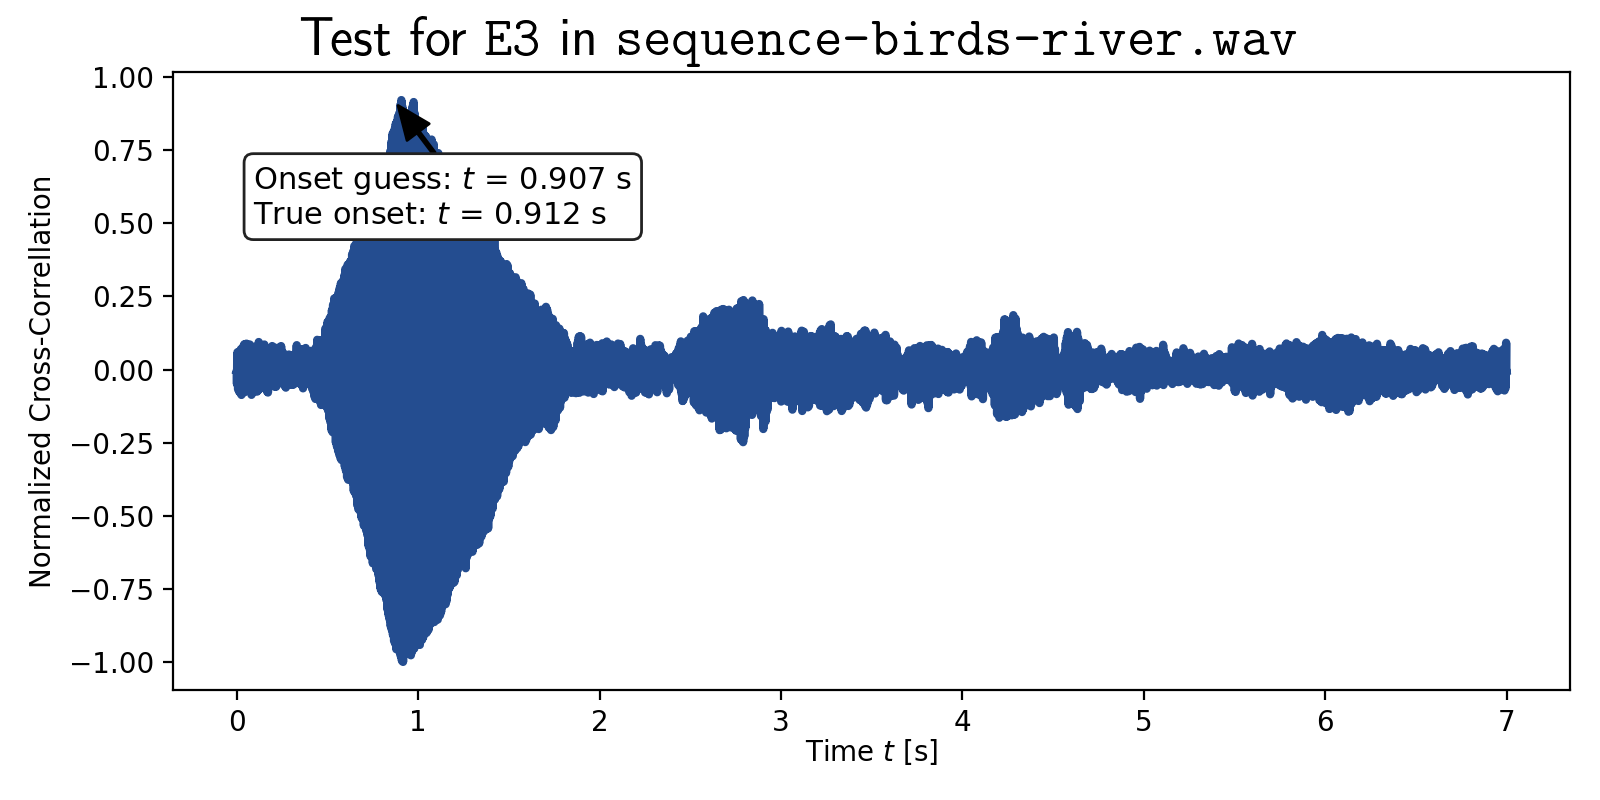
\includegraphics[width=\linewidth]{cross-cor/E3-sequence-birds-river}\vfill  
	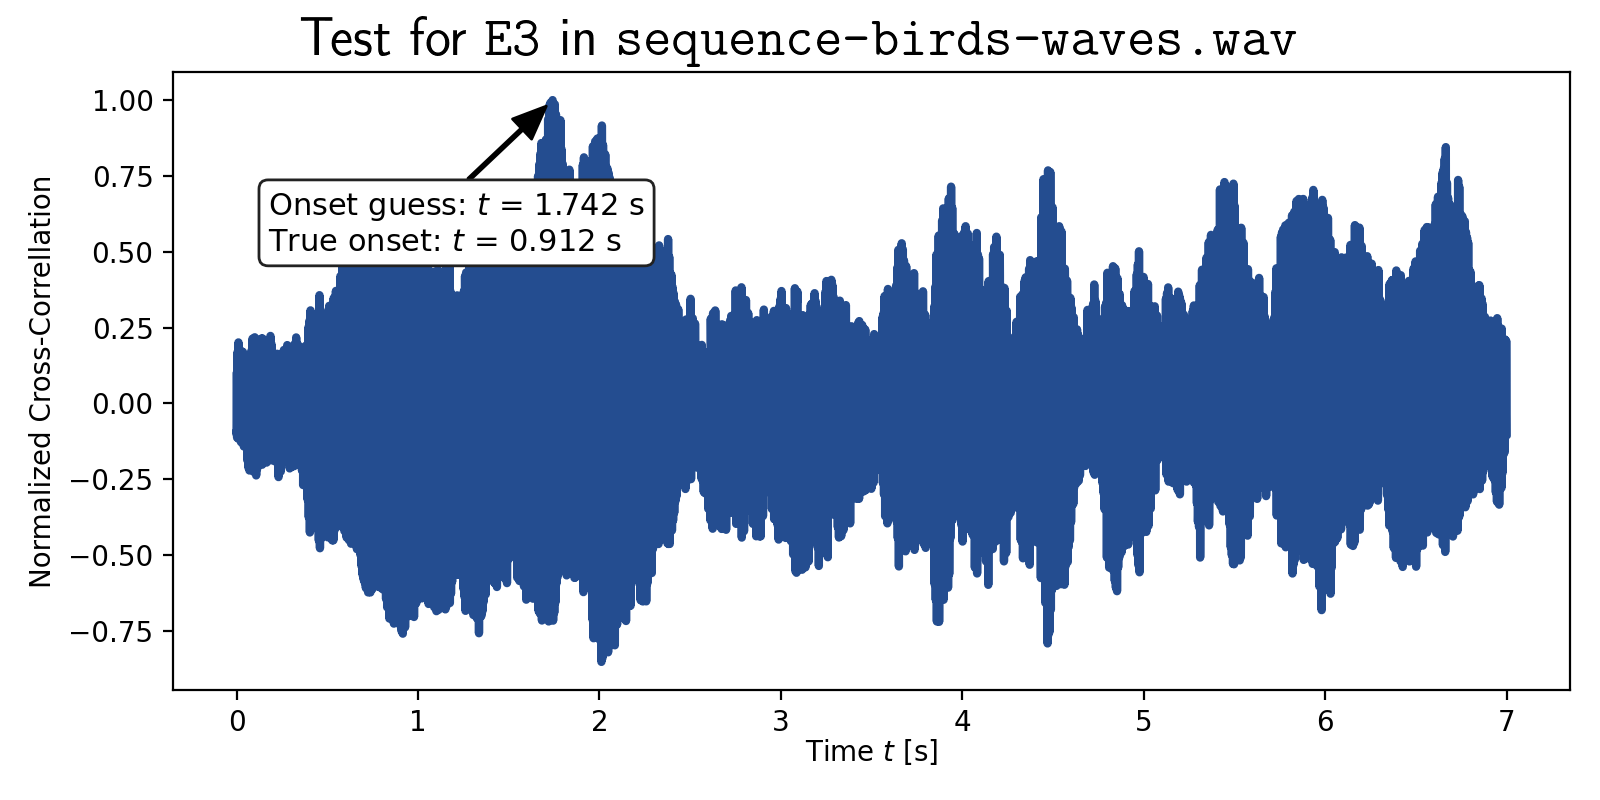
\includegraphics[width=\linewidth]{cross-cor/E3-sequence-birds-waves}\vfill  
	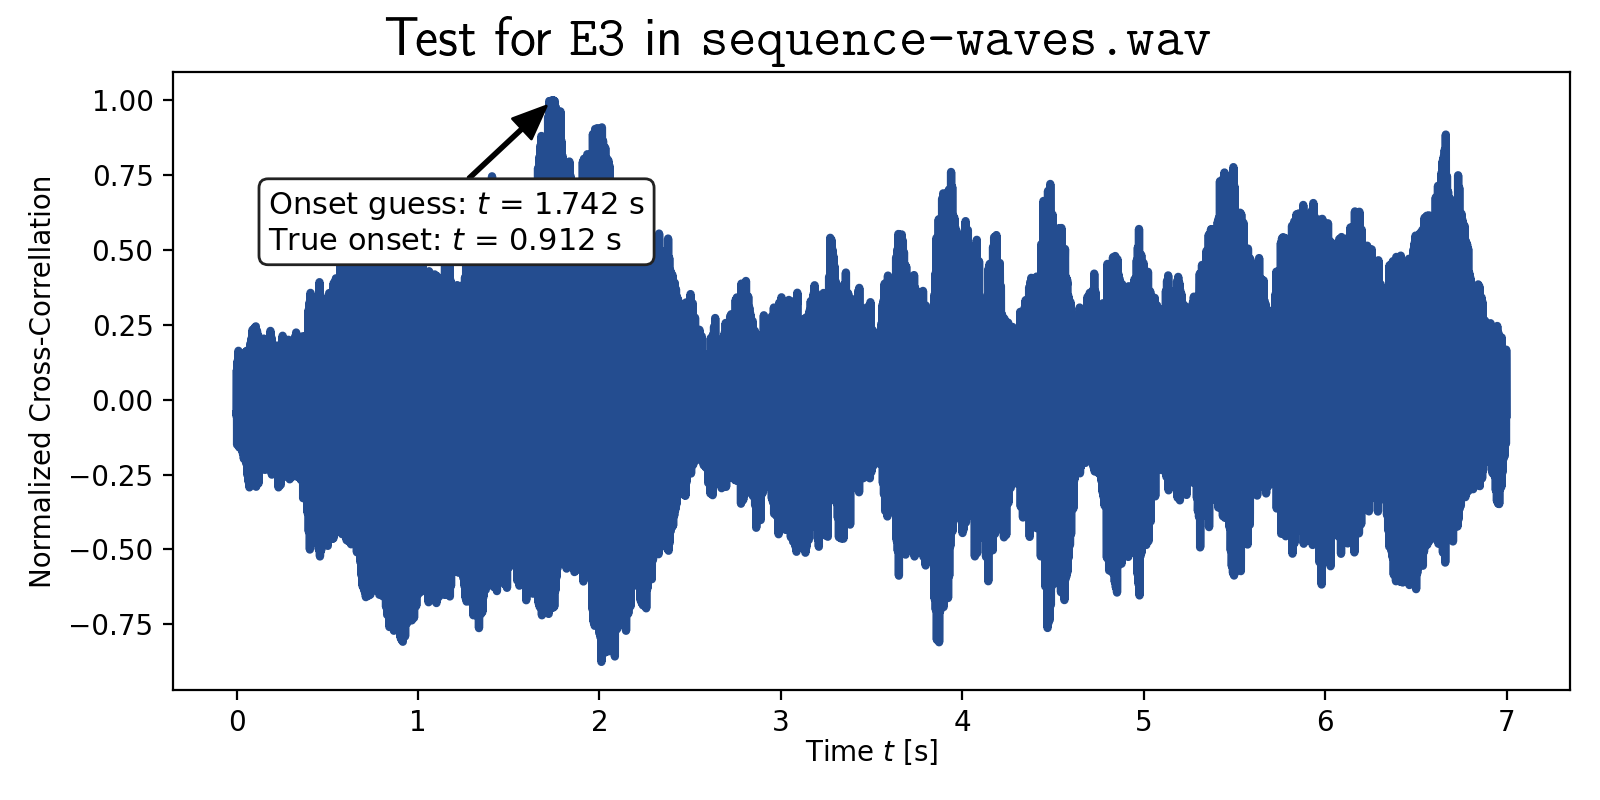
\includegraphics[width=\linewidth]{cross-cor/E3-sequence-waves}\vfill  
	\caption{Using cross-correlation to detect the onset of a faint \texttt{E3} note in a noisy background. Note the method's failure in the last two recordings, but keep in mind that the \texttt{E3} note in particular is excessively faint.}
	\label{fft:fig:E3-crosscor}
\end{figure}

\begin{figure}[htb!]
	\centering
	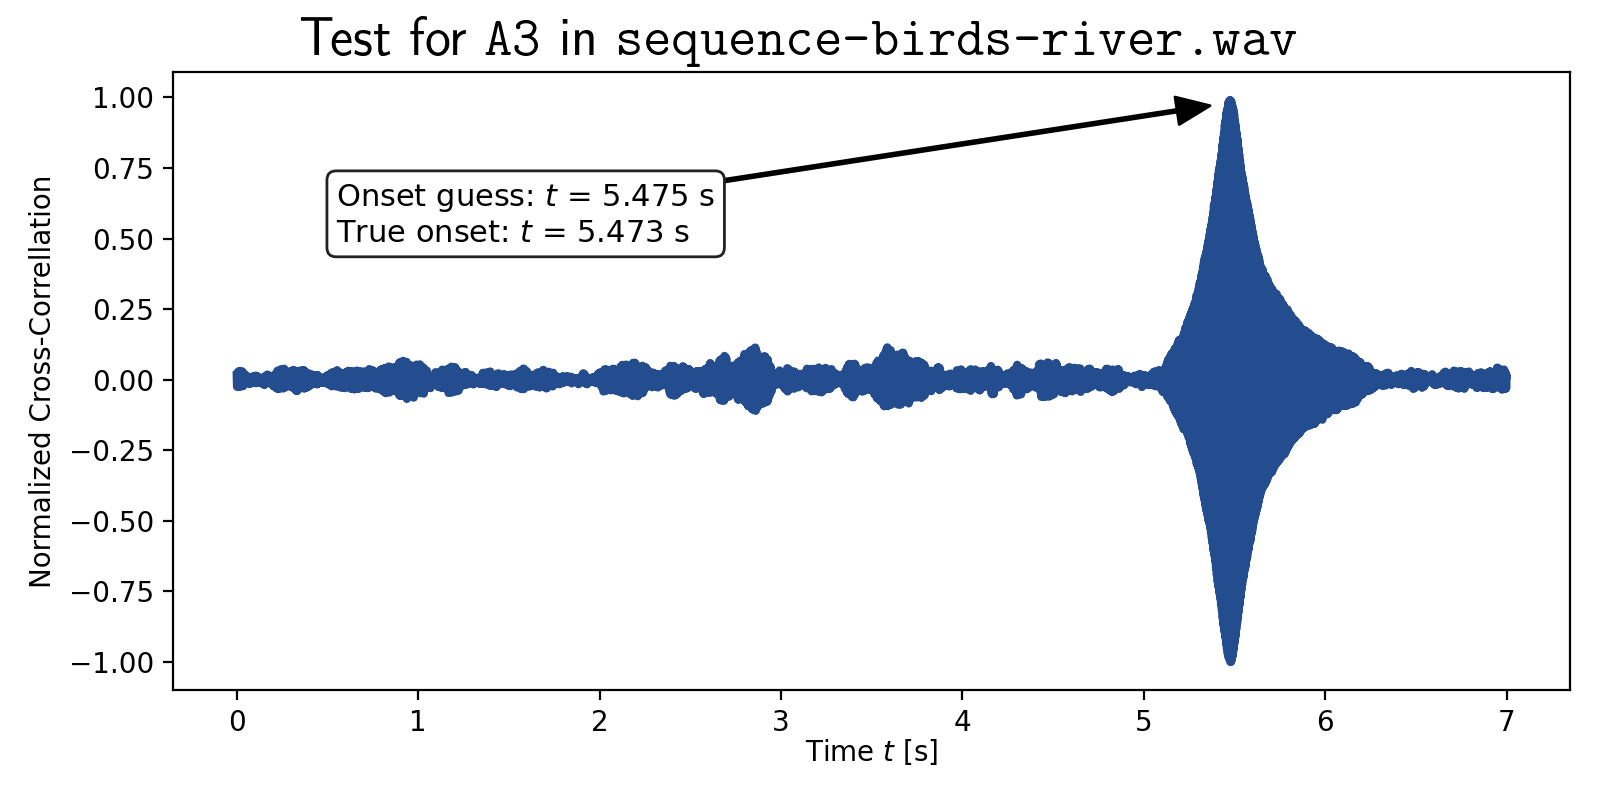
\includegraphics[width=\linewidth]{cross-cor/A3-sequence-birds-river}\vfill  
	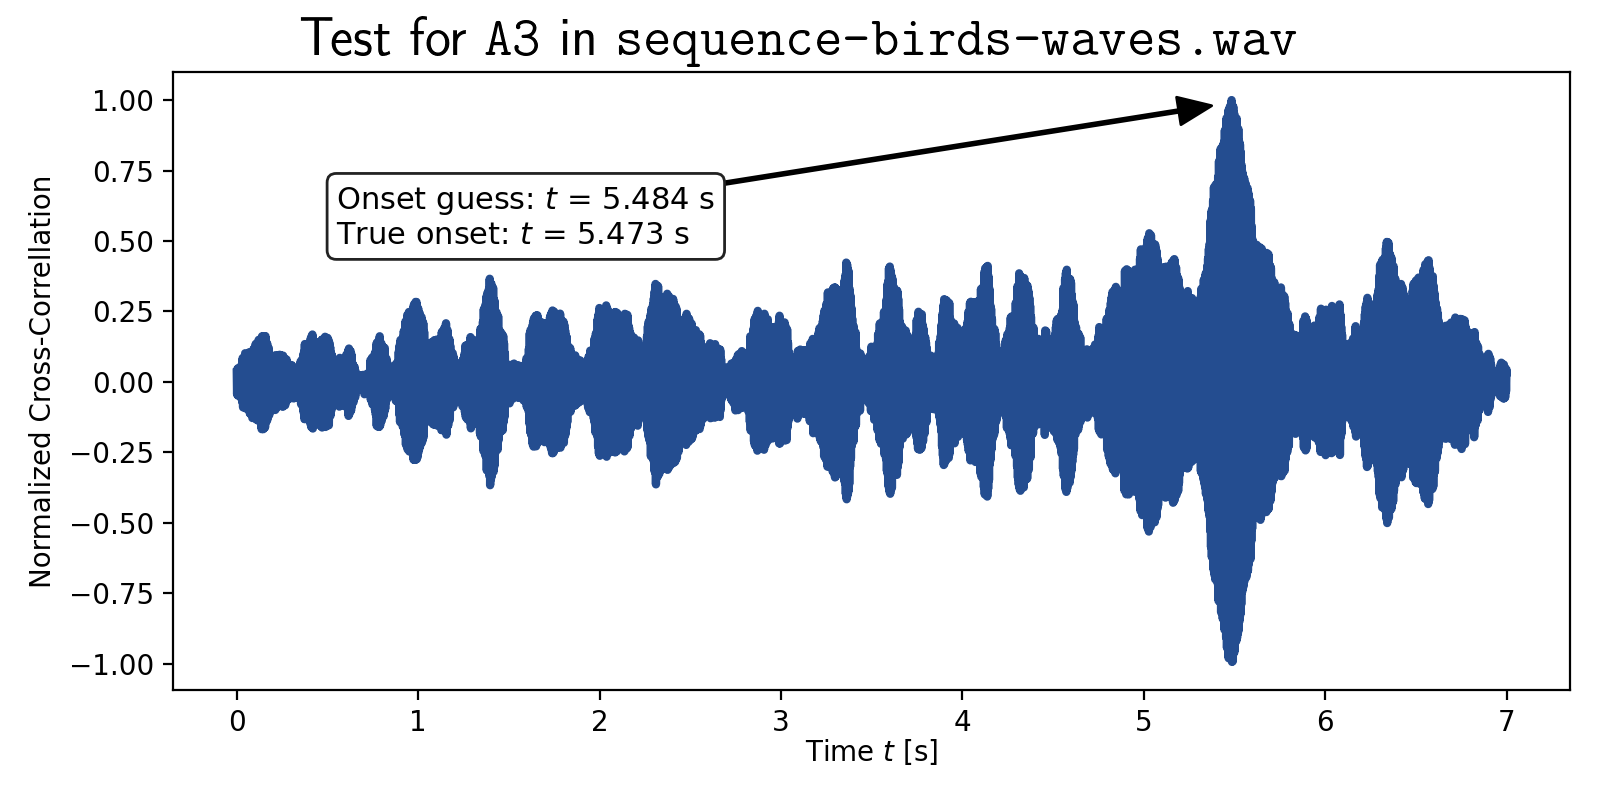
\includegraphics[width=\linewidth]{cross-cor/A3-sequence-birds-waves}\vfill  
	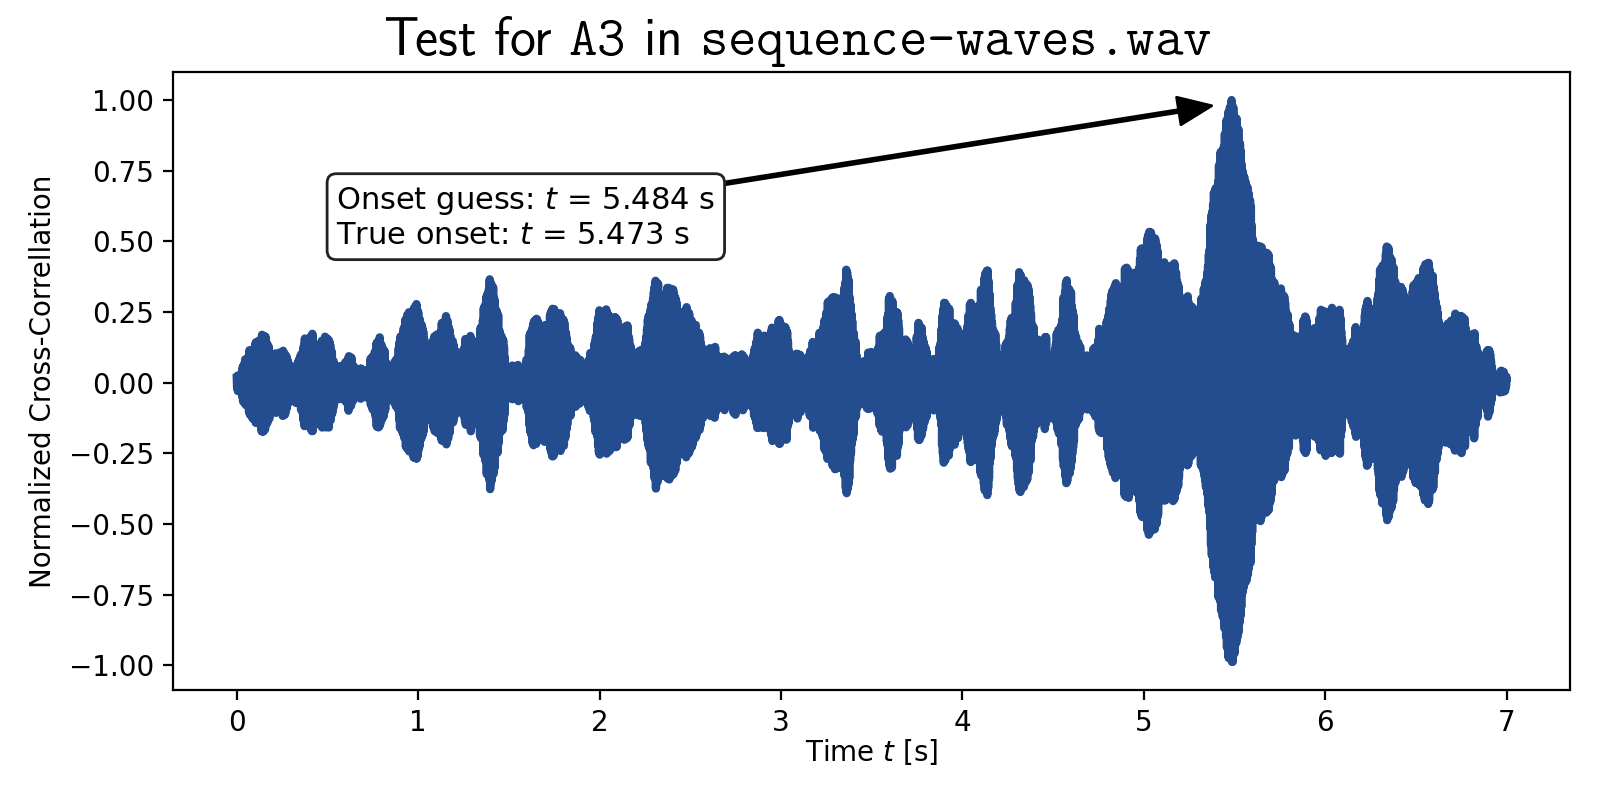
\includegraphics[width=\linewidth]{cross-cor/A3-sequence-waves}\vfill  
	\caption{Using cross-correlation to detect the onset of a faint \texttt{A3} note in a noisy background.}
	\label{fft:fig:A3-crosscor}
\end{figure}


\begin{thebibliography}{}
\setlength{\itemsep}{.2\itemsep}\setlength{\parsep}{.5\parsep}

\bibitem{wiki-cor-cov} Wikipedia contributors. ``Autocorrelation.'' \textit{Wikipedia, The Free Encyclopedia}. 25 October 2020. \url{https://en.wikipedia.org/wiki/Autocorrelation#Normalization}

\bibitem{mit} Derek Rowell. Lecture 22. In \textit{Signal Processing - Continuous and Discrete}---\textit{MIT Course No. 2.161}. Cambridge MA, 2008.
\url{https://ocw.mit.edu/courses/mechanical-engineering/2-161-signal-processing-continuous-and-discrete-fall-2008/lecture-notes/lecture_22.pdf}

\bibitem{autocor-python} Thibauld Nion. ``Autocorrelation functions.'' 2012. \url{https://etudes.tibonihoo.net/literate_musing/autocorrelations.html}. 

\bibitem{horvat} Martin Horvat. ``Avtokorelacijska funckcija''. 2005. \url{https://ucilnica.fmf.uni-lj.si/pluginfile.php/62334/course/section/6936/avtokorelacije.nb.pdf}.

\end{thebibliography}

\end{document}


% Data set with weather: https://machinelearningmastery.com/gentle-introduction-autocorrelation-partial-autocorrelation/


% https://en.wikipedia.org/wiki/String_harmonic